% ===============================
% PROYECTO DEMETER — Documentación Técnica
% Plantilla: ESIBot · Universidad de Sevilla (adaptada)
% Compilar en Overleaf con pdfLaTeX
% ===============================
\documentclass[11pt,a4paper]{report}
\usepackage[spanish, provide=*]{babel}
\usepackage[utf8]{inputenc}
\usepackage[T1]{fontenc}
\usepackage{lmodern}
\usepackage{pdflscape}
\usepackage{fancyhdr}
\usepackage{lastpage}
\usepackage{listings}
\usepackage{xcolor}
\usepackage{amsmath}
\usepackage{graphicx}
\usepackage{titlesec}
\usepackage{hyperref}
\usepackage{booktabs}
\usepackage{array}
\usepackage{float}
\usepackage{caption}
\usepackage{tcolorbox}
\tcbuselibrary{skins, breakable}
\usepackage{longtable}
\usepackage{colortbl}
\usepackage{enumitem}

% ── Geometría ────────────────────────────────────────────────
\usepackage[
    a4paper,
    top=2.5cm,
    bottom=2.5cm,
    left=2cm,
    right=2cm,
    headheight=45pt,
    headsep=15pt,
    footskip=35pt
]{geometry}

% ── Directorio de imágenes ───────────────────────────────────
\graphicspath{{diagrams/}}

% ── Cajas de diseño sin colores ────────────────────────────────
\newenvironment{designnote}
  {\begin{tcolorbox}[colback=white, colframe=black,
     title=Decisión de Diseño, fonttitle=\bfseries, breakable]}
  {\end{tcolorbox}}

\newenvironment{warningbox}
  {\begin{tcolorbox}[colback=white, colframe=black,
     title=Consideración Importante, fonttitle=\bfseries, breakable]}
  {\end{tcolorbox}}

% ── Encabezado páginas normales ──────────────────────────────
\pagestyle{fancy}
\fancyhf{}
\fancyhead[L]{%
  \IfFileExists{diagrams/logo_esibot.png}{%
    
\includegraphics[width=1.5cm]{logo_esibot.png}%
  }{\small\textbf{ESIBot}}%
}
\fancyhead[C]{
    \footnotesize\textbf{Proyecto Demeter} \\
    \scriptsize Plataforma IoT para Investigación Agrícola
}
\fancyhead[R]{
    \footnotesize Daniel Montero Fernández \\
    \scriptsize danmonfer@us.es
}
\fancyfoot[L]{\small Documentación Técnica}
\fancyfoot[C]{\small Página \thepage\ de \pageref{LastPage}}
\fancyfoot[R]{\small Febrero 2026}
\renewcommand{\headrulewidth}{0.4pt}
\renewcommand{\footrulewidth}{0.4pt}

% ── Estilo primera página ────────────────────────────────────
\fancypagestyle{firstpage}{
    \fancyhf{}
    \renewcommand{\headrulewidth}{0.4pt}
    \renewcommand{\footrulewidth}{0.4pt}
    \fancyhead[L]{
\includegraphics[width=2cm]{logo_esibot.png}}
    \fancyhead[C]{
        \normalsize\textbf{Creado por la Asociación Universitaria ESIBot} \\
        \small Correo: esibot@us.es
    }
    \fancyhead[R]{
        \small Autor: Daniel Montero Fernández \\
        \small Correo: danmonfer@us.es \\
        \small Fecha: Febrero 2026
    }
    \fancyfoot[L]{\small Documentación Técnica - Proyecto Demeter}
    \fancyfoot[C]{\small Página \thepage\ de \pageref{LastPage}}
    \fancyfoot[R]{\small 11 de febrero de 2026}
}

% ── Listings ─────────────────────────────────────────────────
\lstdefinestyle{trama}{
    basicstyle=\ttfamily\small,
    backgroundcolor=\color{gray!10},
    frame=single,
    breaklines=true,
    columns=fullflexible
}

% ── Formato de secciones ─────────────────────────────────────
\titleformat{\chapter}[display]{\normalfont\huge\bfseries}{\chaptertitlename\ \thechapter}{20pt}{\Huge}
\titleformat{\section}{\normalfont\Large\bfseries}{\thesection}{1em}{}
\titleformat{\subsection}{\normalfont\large\bfseries}{\thesubsection}{1em}{}
\titleformat{\subsubsection}{\normalfont\normalsize\bfseries}{\thesubsubsection}{1em}{}

% ── Hipervínculos ────────────────────────────────────────────
\hypersetup{
    colorlinks=true,
    linkcolor=blue!60!black,
    urlcolor=blue,
    citecolor=green!50!black,
    pdftitle={Proyecto Demeter --- Documentación Técnica},
    pdfauthor={Daniel Montero Fernández}
}

% ============================================================
\begin{document}

% ── Portada ──────────────────────────────────────────────────
\thispagestyle{firstpage}
\begin{center}
    \vspace*{1cm}
    
    % Logo
    
\includegraphics[width=0.35\textwidth]{logo_esibot.png}
    
    \vspace{1cm}
    
    % Título principal
    {\Huge \textbf{Proyecto DEMETER}}
    
    \vspace{0.5cm}
    
    % Subtítulo
    {\Large Plataforma Integral de Monitorización y Gestión\\
    para Investigación Agrícola}
    
    \vspace{0.4cm}
    {\large \textit{IoT · Firmware ESP32 · Backend FastAPI · LIMS}}
    
    \vspace{1.2cm}
    \rule{\textwidth}{1pt}
    \vspace{0.4cm}
    
    {\LARGE \textbf{Documentación Técnica del Sistema}}
    
    \vspace{0.4cm}
    \rule{\textwidth}{1pt}
    
    \vfill
    
    \begin{tabular}{rl}
        \textbf{Autor:}        & Daniel Montero Fernández \\[0.3cm]
        \textbf{Contacto:}      & danmonfer@us.es \\[0.3cm]
        \textbf{Institución:}   & Universidad de Sevilla \\[0.3cm]
        \textbf{Versión:}       & 1.0 \\[0.3cm]
        \textbf{Fecha:}         & Febrero de 2026 \\[0.3cm]
        \textbf{Estado:}        & En desarrollo activo \\
    \end{tabular}
    
    \vspace{1.5cm}
    {\small Este documento es confidencial y de uso interno del proyecto.}
\end{center}

\newpage

% ── Índice ───────────────────────────────────────────────────
\pagestyle{fancy}
\tableofcontents
\newpage

% ============================================================
% CAPÍTULOS PRINCIPALES
% ============================================================
% ============================================================
% SECCIÓN 1: Introducción y Visión del Proyecto
% ============================================================
\chapter*{Introducción y Visión del Proyecto}
\addcontentsline{toc}{chapter}{Introducción y Visión del Proyecto}

% ─────────────────────────────────────────────────────────────
\section{Origen del Proyecto}

El \textbf{Proyecto Demeter} nace en el seno de la asociación universitaria
\textbf{ESIBot} (Escuela Técnica Superior de Ingeniería, Universidad de Sevilla)
como un ejercicio de ingeniería full-stack aplicada a un dominio físico real:
la monitorización y el control automatizado de entornos de cultivo. Su autor,
Daniel Montero Fernández, conduce el proyecto en solitario a lo largo de
varias iteraciones, partiendo de una primera prueba de concepto sobre Arduino
y evolucionando hasta la arquitectura distribuida documentada en este texto:
una red de microcontroladores ESP32, un servicio de borde sobre Raspberry Pi,
un servidor central desplegable indistintamente en Google Cloud Platform o en
hardware doméstico, y un SDK científico de Python para análisis agronómico.

La presente versión 1.0 marca el cierre del ciclo de desarrollo activo del
proyecto. Se entrega como \textit{release} estable y \textit{portfolio
piece}, no como abandono: el sistema queda funcional, documentado y
reproducible, con una cláusula explícita de no continuidad (\textit{no further
development planned}) que libera al autor del compromiso de mantenimiento
indefinido y, simultáneamente, fija el alcance de lo entregado.

% ─────────────────────────────────────────────────────────────
\section{Motivación}

La monitorización continua de variables ambientales y la trazabilidad de los
sujetos experimentales son requisitos básicos en cualquier protocolo
agronómico riguroso, pero su implantación en pequeños invernaderos de
investigación universitaria choca con dos limitaciones recurrentes: la
\textbf{necesidad de presencia humana} para tomar lecturas y operar el riego,
y el \textbf{coste de las plataformas comerciales} de gestión de información
de laboratorio (LIMS), normalmente diseñadas para entornos clínicos o
industriales y desproporcionadas para grupos pequeños. Demeter aborda ambos
frentes con hardware de bajo coste, software libre y un alcance
deliberadamente acotado.

% ─────────────────────────────────────────────────────────────
\section{Objetivos del Sistema}

\subsection{Objetivo General}
Desarrollar una plataforma IoT integral que permita monitorizar, controlar y
analizar entornos de cultivo, proporcionando trazabilidad científica completa
de las plantas y los experimentos asociados.

\subsection{Objetivos Específicos}

Estos cuatro objetivos articulan el resto del documento y se retoman en el
Capítulo~\ref{sec:conclusiones} para evaluar el grado de cumplimiento de
la versión 1.0:

\begin{itemize}[leftmargin=*, label=--]
    \item \textbf{Automatización IoT.} Desplegar una red de sensores de bajo
          coste y alta fiabilidad que recolecte variables ambientales de
          forma continua y sin intervención humana.
    \item \textbf{Control Remoto.} Permitir la actuación sobre los elementos
          físicos del entorno (bombas de riego, electroválvulas, ventanas)
          desde cualquier punto con acceso a internet.
    \item \textbf{Trazabilidad LIMS.} Implementar un sistema de gestión de
          información de laboratorio que mantenga un registro estructurado
          de cada planta y los experimentos en los que participa.
    \item \textbf{Análisis Científico.} Dotar a los investigadores de
          herramientas (SDK, gráficas, informes exportables) para extraer y
          analizar datos sin depender del equipo de soporte técnico.
\end{itemize}

% ─────────────────────────────────────────────────────────────
\section{Alcance del Documento}

Este documento es la \textbf{documentación técnica de arquitectura} del
sistema Demeter. Su audiencia objetivo son personas con perfil técnico
(desarrolladores, evaluadores, mantenedores futuros) que necesitan entender
\textit{cómo está construido} el sistema, \textit{por qué se tomaron las
decisiones} de diseño que se tomaron, y \textit{cómo desplegarlo} desde un
entorno limpio.

\textbf{Lo que cubre este documento:}

\begin{itemize}[leftmargin=*, label=--]
    \item Arquitectura de cada una de las cuatro capas del sistema y de las
          fronteras entre ellas (Capítulos~\ref{sec:protocolo} a \ref{sec:sdk}).
    \item Estrategia de validación y banco de tests automatizados verificable
          (Capítulo~\ref{sec:testing}).
    \item Procedimiento reproducible de despliegue en los cuatro entornos
          soportados, incluyendo CI/CD y operaciones
          (Capítulo~\ref{sec:despliegue}).
    \item Estado de la versión 1.0 y lecciones aprendidas
          (Capítulo~\ref{sec:conclusiones}).
\end{itemize}

\textbf{Lo que NO cubre este documento} (y dónde encontrarlo):

\begin{itemize}[leftmargin=*, label=--]
    \item \textbf{Manual de usuario final}: cómo usar el dashboard, cómo crear
          un experimento, cómo interpretar las gráficas. La interfaz se
          documenta en el propio frontend mediante \textit{tooltips}, ayudas
          contextuales y un README específico del módulo.
    \item \textbf{Informe de viabilidad y cierre del proyecto}: análisis de
          sostenibilidad económica, justificación del cierre como v1.0
          \textit{release} y plan de entrega académica. Documento separado en
          \texttt{docs/Closure/LaTeX/main.pdf}.
    \item \textbf{Guías de desarrollo de plugins o módulos terceros}: la
          versión 1.0 no contempla extensibilidad mediante plugins. Una
          eventual versión futura debería añadir esta dimensión a la
          documentación.
\end{itemize}

% ─────────────────────────────────────────────────────────────
\section{Glosario y Siglas}

A lo largo del documento se emplean los siguientes términos y siglas, muchos
de los cuales son habituales en sus dominios respectivos pero pueden requerir
contextualización conjunta.

\begin{table}[H]
    \centering
    \caption{Glosario de términos y siglas empleados en el documento}
    \begin{tabularx}{\textwidth}{lX}
        \toprule
        \textbf{Sigla / Término}      & \textbf{Significado y contexto en Demeter} \\
        \midrule
        ADR                            & \textit{Architecture Decision Record}. Registro corto que documenta una decisión arquitectónica relevante, sus alternativas y su justificación. \\
        API REST                       & \textit{Application Programming Interface} sobre HTTP siguiendo el estilo arquitectónico REST. \\
        CRC                            & \textit{Cyclic Redundancy Check}. Suma de verificación que protege la integridad de las tramas del protocolo binario Demeter. \\
        ESP-NOW                        & Protocolo de comunicación inalámbrica entre dispositivos ESP32 sin necesidad de un punto de acceso WiFi. \\
        ET\textsubscript{0}            & \textit{Evapotranspiración de referencia}. Indicador agronómico que estima la pérdida de agua del cultivo por unidad de tiempo. \\
        GDD                            & \textit{Growing Degree Days}. Acumulado térmico que se usa para predecir fases fenológicas del cultivo. \\
        IoT                            & \textit{Internet of Things}. Paradigma de dispositivos físicos conectados que recolectan y reaccionan a datos del entorno. \\
        JWT                            & \textit{JSON Web Token}. Formato compacto de token firmado usado para autenticación entre el frontend y el backend. \\
        LIMS                           & \textit{Laboratory Information Management System}. Sistema que organiza la trazabilidad de muestras y experimentos en un laboratorio. \\
        OTA                            & \textit{Over-The-Air}. Actualización remota del firmware sin intervención física sobre el dispositivo. NO implementado en v1.0. \\
        Parquet                        & Formato columnar de almacenamiento de datos usado por el SDK como caché local de telemetría. \\
        RBAC                           & \textit{Role-Based Access Control}. Modelo de control de acceso basado en roles (admin, viewer) usado por el backend. \\
        RQ                             & \textit{Redis Queue}. Librería Python que implementa una cola de tareas asíncronas sobre Redis, usada por el \textit{math worker}. \\
        SDK                            & \textit{Software Development Kit}. En Demeter, el paquete Python \texttt{demeter\_sdk} que provee acceso programático a la plataforma. \\
        TLS                            & \textit{Transport Layer Security}. Cifrado del transporte HTTPS y WebSocket Seguro (WSS). \\
        UART                           & \textit{Universal Asynchronous Receiver-Transmitter}. Enlace serie entre el ESP32 \textit{gateway} y la Raspberry Pi. \\
        VPD                            & \textit{Vapor Pressure Deficit}. Indicador agronómico que cuantifica el estrés hídrico atmosférico sobre la planta. \\
        WSS                            & \textit{WebSocket Secure}. WebSocket sobre TLS, transporte usado entre la Raspberry Pi y el backend. \\
        \bottomrule
    \end{tabularx}
    \label{tab:glosario}
\end{table}

\newpage
% ============================================================
% SECCIÓN 3: Protocolo Demeter
% ============================================================
\chapter{Protocolo de Comunicación Demeter}
\label{sec:protocolo}

\section{Propósito y Filosofía de Diseño}

El Protocolo Demeter es un protocolo de comunicación binario diseñado específicamente para
la red de campo del sistema. Los protocolos estándar de texto (JSON, CSV) son demasiado
pesados para microcontroladores con memoria limitada y canales de radio estrecho. Un paquete
JSON con temperatura y humedad puede ocupar entre 40 y 80 bytes. La misma información en
el Protocolo Demeter ocupa exactamente \textbf{10 bytes}.

\begin{designnote}
Las decisiones de diseño que guían el protocolo son: \textbf{compacidad} (cada bit cuenta),
\textbf{determinismo} (la longitud de cada trama es conocida antes de recibirla),
\textbf{robustez} (verificación de integridad en toda trama) y
\textbf{extensibilidad} (hasta 254 tipos de mensaje sin modificar la estructura base).
\end{designnote}

% ─────────────────────────────────────────────────────────────
\section{Modelos Pydantic: Bridging entre Binario y JSON}
\label{sec:pydantic}

Una aportación central de la arquitectura Demeter es que el protocolo no es exclusivamente
binario: las mismas definiciones de mensaje coexisten en \textbf{dos representaciones},
gestionadas mediante \textbf{modelos Pydantic} validados y tipados:

\begin{enumerate}
    \item \textbf{Representación JSON}: usada en la comunicación entre el Frontend y el
          Backend por HTTP y WebSocket. Los campos viajan con sus nombres completos
          (e.g. \texttt{"type"}, \texttt{"target\_id"}, \texttt{"pin"}, \texttt{"value"}).
    \item \textbf{Representación Binaria}: usada en la comunicación de red de campo
          (UART entre Raspberry Pi y Gateway, y ESP-NOW entre nodos). Solo los valores
          numéricos viajan en la trama; los nombres de campo \textit{no existen en el paquete},
          reduciéndolo a su mínima expresión.
\end{enumerate}

\subsection{Diseño de Modelos Discriminados}

Cada tipo de comando del protocolo tiene su propio modelo Pydantic con un campo
\texttt{type} que actúa como \textbf{discriminador de unión}. Esto permite que al
deserializar un JSON, Pydantic identifique automáticamente de qué tipo de mensaje
se trata y lo valide con el esquema apropiado:

\begin{lstlisting}[style=trama, caption={Estructura conceptual de un modelo discriminado}]
{
  "type": "set_gpio",   <-- discriminador: identifica el subtipo exacto
  "target_id": 3,       <-- nodo destino
  "pin": 4,             <-- pin a controlar
  "value": 1,           <-- 1=ON, 0=OFF
  "duration_ms": 15000  <-- tiempo de activacion (ms)
}
\end{lstlisting}

La clave del diseño es que el campo \texttt{type} es unívoco por subtipo. Cuando el
Backend recibe este JSON (desde el Frontend o la API), instancia mediante
\texttt{TypeAdapter[AnyDemeterCommand]} el modelo correcto sin lógica condicional manual.

\subsection{Auto-descubrimiento y Clasificación Automática}

El uso del patrón de \textbf{unión discriminada} con Pydantic permite que cualquier capa
del sistema clasifique un mensaje desconocido sin necesidad de \textit{switch-case} explícitos:
la librería inspecciona el campo \texttt{type} y devuelve la instancia del modelo correcto,
ya validada y tipada. Esto tiene tres consecuencias importantes:

\begin{itemize}[leftmargin=*, label=--]
    \item \textbf{Validación zero-cost}: si un campo falta o tiene tipo incorrecto,
          Pydantic lanza una excepción detallada antes de que el sistema procese nada.
    \item \textbf{Serialización simétrica}: \texttt{model.model\_dump\_json()} produce el
          JSON que el Frontend espera; \texttt{model.to\_binary()} produce la trama que
          el ESP32 espera. La lógica de transformación reside en el modelo, no en el
          controlador.
    \item \textbf{Reutilización del esquema}: el mismo \texttt{Common/schemas.py} es
          importado por el Backend (Python) y puede referenciarse para generar SDKs cliente,
          documentación automática (OpenAPI) o tests de integración.
\end{itemize}

\subsection{Conversión Binaria: Solo los Valores}

La diferencia fundamental entre JSON y binario es que en la trama física
\textbf{los nombres de los campos no existen}. El orden y tamaño de cada byte es implícito
al tipo de comando (definido por el \texttt{CMD\_ID} de la cabecera). Por ejemplo, para un
\texttt{SET\_GPIO} el payload es exactamente 3 bytes: \texttt{[PIN, VALUE, FLAGS]}.

La serialización binaria rellena cada byte en orden, con el tamaño y signo definidos por
el esquema del protocolo (enteros sin signo, punt fijo para float, Little Endian).

% ─────────────────────────────────────────────────────────────
\section{Comunicación HTTP y WebSocket en el Sistema}
\label{sec:http_ws}

\subsection{Flujo de un Comando desde el Navegador}

Cuando un operador interactúa con el dashboard activo, los comandos siguen un flujo
completamente desacoplado de la red de campo:

\begin{enumerate}
    \item El \textbf{Frontend React} compone un objeto JSON conforme al esquema del modelo
          Pydantic correspondiente (e.g. \texttt{set\_gpio}) y lo envía mediante una petición
          \textbf{HTTP POST} a \texttt{/api/command}.
    \item El \textbf{Backend FastAPI} recibe el JSON, lo valida automáticamente con el
          \texttt{TypeAdapter} discriminado, y publica el comando en el canal Redis
          \texttt{demeter:commands}. Devuelve \texttt{202 Accepted} inmediatamente.
    \item El \textbf{WS Dispatcher} (tarea asyncio en el Backend) consume el mensaje de Redis
          y lo retransmite por WebSocket a la Raspberry Pi, identificada como
          \texttt{raspberry\_gateway}.
    \item La \textbf{Raspberry Pi} recibe el JSON por WebSocket, lo convierte a trama binaria
          mediante el mismo modelo Pydantic en Python, y lo envía por UART al Gateway ESP32.
    \item El \textbf{Gateway ESP32} reenvía la trama binaria por ESP-NOW al nodo actuador
          destino, que ejecuta la acción y confirma con \texttt{CMD\_ACK}.
\end{enumerate}

\subsection{Flujo de Telemetría en Tiempo Real}

El camino inverso (del sensor al dashboard) funciona de forma reactiva:

\begin{enumerate}
    \item El \textbf{Nodo Sensor} emite tramas binarias por ESP-NOW en el intervalo configurado.
    \item El \textbf{Gateway ESP32} las reenvía por UART a la Raspberry Pi.
    \item La \textbf{Raspberry Pi} las decodifica (Protocolo Demeter en Python), construye un
          JSON y lo publica por WebSocket hacia el Backend.
    \item El \textbf{Backend} almacena la medición en Redis (caché 60~s) y en PostgreSQL
          (persistencia), y hace \textit{broadcast} por WebSocket a todos los clientes
          Frontend suscritos.
    \item El \textbf{Frontend} recibe el push y actualiza los gráficos sin ninguna petición
          adicional por parte del usuario.
\end{enumerate}

\begin{designnote}
\textbf{Separación de canales}: Los comandos viajan por \textbf{HTTP POST} (fiables, con
respuesta de estado). La telemetría viaja por \textbf{WebSocket} (baja latencia, push).
Para la Raspberry Pi, el canal WebSocket es exclusivo y bidireccional. Para el Frontend,
el WebSocket es de solo lectura; sus comandos siempre van por HTTP.
\end{designnote}

% ─────────────────────────────────────────────────────────────
\section{Estructura de una Trama}

Toda comunicación sigue el mismo formato de cabecera fija seguida de un payload variable:

\begin{table}[H]
    \centering
    \caption{Campos de la cabecera Demeter}
    \begin{tabular}{clp{8cm}}
        \toprule
        \textbf{Campo}  & \textbf{Tamaño} & \textbf{Descripción} \\
        \midrule
        SYNC    & 1 byte & Siempre \texttt{0xAA}. Marca el inicio de cualquier trama válida. \\
        FLAGS   & 1 byte & Reservado. Actualmente \texttt{0x00}. \\
        SRC\_ID & 1 byte & Identificador numérico del nodo emisor (1--253). \\
        DST\_ID & 1 byte & Destino: \texttt{0x00}=servidor, \texttt{0xFF}=difusión. \\
        CMD\_ID & 1 byte & Tipo de mensaje (ver catálogo). \\
        LENGTH  & 1 byte & Número de bytes del payload (0--255). \\
        PAYLOAD & N bytes & Datos específicos del tipo de mensaje, formato Little Endian. \\
        CRC     & 1 byte & Suma módulo 256 de FLAGS hasta fin del payload. \\
        \bottomrule
    \end{tabular}
    \label{tab:cabecera_demeter}
\end{table}

\textbf{Tamaños:} mínimo 7 bytes (sin payload) · máximo teórico 262 bytes · típico 10--14 bytes.

% ─────────────────────────────────────────────────────────────
\section{Catálogo de Mensajes}

\begin{table}[H]
    \centering
    \caption{Catálogo completo de comandos del Protocolo Demeter v2}
    \begin{tabular}{clcp{5cm}}
        \toprule
        \textbf{CMD\_ID} & \textbf{Nombre} & \textbf{Payload (bytes)} & \textbf{Descripción} \\
        \midrule
        \texttt{0x01} & PING            & 0  & Keep-alive. Espera ACK. \\
        \texttt{0x02} & ACK             & 0--1 & Confirmación con contexto de sesión opcional. \\
        \texttt{0x03} & NACK            & 1  & Rechazo con código de error. \\
        \texttt{0x04} & SYN             & 0  & Inicio del handshake (paso 1/3). \\
        \texttt{0x05} & SYN-ACK         & 0  & Confirmación de disponibilidad (paso 2/3). \\
        \texttt{0x0A} & ROUTE\_ADD      & 7  & Registra una nueva ruta en la tabla del Gateway. \\
        \texttt{0x0B} & TEMP\_HUM\_REPORT & 4 & Datos de temperatura y humedad (punto fijo ×100). \\
        \texttt{0x0C} & PIN\_REPORT     & 2  & Estado de un pin tras ejecución de un comando. \\
        \texttt{0x0D} & SYSTEM\_REPORT  & 8  & Modo de operación y nivel de batería en mV. \\
        \texttt{0x10} & SET\_GPIO       & 3  & Orden de cambio de estado de un pin. \\
        \texttt{0x11} & SET\_PWM        & 3  & Señal analógica (control de velocidad/intensidad). \\
        \texttt{0x20} & GET\_SENSORS    & 0  & Solicitud de lectura inmediata de sensores. \\
        \texttt{0x30} & EXEC\_SEQUENCE  & Variable & Lista de pasos de actuación con temporización. \\
        \bottomrule
    \end{tabular}
    \label{tab:catalogo_comandos}
\end{table}

% ─────────────────────────────────────────────────────────────
\section{Codificación de Datos}

\subsection{Temperatura y Humedad (Punto Fijo ×100)}

Los valores se multiplican por 100 y se codifican como enteros con signo de 16 bits
en formato Little Endian:

\[
T = 24{,}57\,^{\circ}\text{C} \rightarrow 2457 = \texttt{0x0999} \rightarrow \text{bytes: } \texttt{[99\;09]}
\]
\[
H = 63{,}20\,\% \rightarrow 6320 = \texttt{0x18B0} \rightarrow \text{bytes: } \texttt{[B0\;18]}
\]

\subsection{Duraciones en Secuencias (32 bits Little Endian)}

Las duraciones se expresan en milisegundos como entero de 32 bits sin signo:
\[
2500\,\text{ms} = \texttt{0x000009C4} \rightarrow \text{bytes: } \texttt{[C4\;09\;00\;00]}
\]

% ─────────────────────────────────────────────────────────────
\section{Ejemplos de Tramas Reales}

\subsection{Telemetría de Sensor (TEMP\_HUM\_REPORT)}
Nodo 2 envía T=24,57°C y H=63,20\% al servidor:

\begin{lstlisting}[style=trama, caption={Trama TEMP\_HUM\_REPORT completa}]
Pos: [0]   [1]   [2]   [3]   [4]   [5]   [6]   [7]   [8]   [9]
Hex: AA     00    02    00    0B    04    99    09    B0    18   CRC
     SYNC  FLAGS  SRC   DST   CMD   LEN  T_Lo  T_Hi  H_Lo  H_Hi
                  (2)   (0) TH_RPT  (4)  ---- 24.57 C ----  -63.20%-
\end{lstlisting}

\subsection{Comando de Actuación (SET\_GPIO)}
Servidor ordena al nodo 3 encender el pin 4 (bomba):

\begin{lstlisting}[style=trama, caption={Trama SET\_GPIO}]
Pos: [0]   [1]   [2]   [3]   [4]   [5]   [6]   [7]   [8]   [9]
Hex: AA     00    00    03    10    03    04    01    00    CRC
     SYNC  FLAGS  SRC   DST   CMD   LEN   PIN  VAL  FLAGS
                  (0)   (3) SET_IO  (3)   (4) HIGH    (0)
\end{lstlisting}

\subsection{Inicio de Handshake (SYN)}
Nodo sensor 2 solicita sesión con el Gateway (nodo 1):

\begin{lstlisting}[style=trama, caption={Trama SYN mínima --- 7 bytes}]
Pos: [0]   [1]   [2]   [3]   [4]   [5]   [6]
Hex: AA     00    02    01    04    00    CRC
     SYNC  FLAGS  SRC   DST   CMD   LEN
                  (2)   (1)   SYN   (0)
\end{lstlisting}

% ─────────────────────────────────────────────────────────────
\section{Algoritmos de Serialización y Deserialización}

\subsection{Serialización}

El proceso de serialización transforma los datos de aplicación en una trama binaria
completamente estructurada. Toma el comando o reporte, convierte sus campos al
formato numérico requerido (punto fijo para temperatura, Little Endian para enteros),
construye el payload en un buffer, prepende la cabecera y calcula el CRC.

\subsection{Deserialización y Validación}

El \textit{pipeline} de deserialización actúa como barrera de seguridad: verifica
progresivamente el byte de inicio (SYNC), la longitud declarada, el CRC y el destino.
Solo si todas las comprobaciones pasan se decodifica el payload y se lanza el evento
interno asociado al tipo de mensaje.

\subsection{Manejo de Errores}

\begin{warningbox}
El protocolo adopta la filosofía de \textbf{fallo silencioso}: una trama corrupta no genera
ninguna respuesta de error. Esto evita tormentas de retroalimentación ante interferencias de
radio. El NACK se reserva para errores de lógica de aplicación (pin no válido, modo IDLE activo).
\end{warningbox}

% ─────────────────────────────────────────────────────────────
\section{Handshake TCP-like}

Antes de operar, cada nodo negocia una sesión con el Gateway mediante un triple
\textit{handshake}: el emisor envía SYN, espera SYN-ACK con \textit{timeout} de 2~s
y hasta 3 reintentos, y confirma con ACK. Solo tras este acuerdo comienzan los reportes.

% ─────────────────────────────────────────────────────────────
\section{Flujo Extremo a Extremo}

Una trama parte del Nodo Sensor en formato binario por ESP-NOW, llega al Gateway,
se reenvía por UART a la Raspberry Pi, que la decodifica y publica como JSON al Backend.
El Backend la persiste en PostgreSQL y distribuye en tiempo real a todos los clientes
conectados por WebSocket, con reacción visual a la décima de segundo.

% ─────────────────────────────────────────────────────────────
\section{Consideraciones de Tiempo y Saturación}

\subsection{Tiempos de Transmisión}

\begin{table}[H]
    \centering
    \caption{Parámetros de tiempo de transmisión del protocolo}
    \begin{tabular}{lc}
        \toprule
        \textbf{Parámetro} & \textbf{Valor} \\
        \midrule
        Tiempo de transmisión por trama (10B) & $\approx$ 0,5 ms \\
        Latencia extremo a extremo (RF + serial) & 3 -- 10 ms \\
        Intervalo de reporte del sensor (configurado) & 5.000 ms \\
        Ocupación del canal por nodo sensor & < 0,01\% \\
        \bottomrule
    \end{tabular}
    \label{tab:tiempos}
\end{table}

\subsection{Ciclo Energético del Nodo Sensor}

El nodo sensor efectúa un intenso ahorro de recursos invocando Deep Sleep del ESP32 entre
reportes. Un nodo configurado con reportes cada 60~s puede operar durante más de un año
con una batería de 3000 mAh.

\begin{warningbox}
Los nodos actuadores y el Gateway deben permanecer activos de forma continua y requieren
alimentación estable. Solo el Nodo Sensor puede operar con batería durante periodos prolongados.
\end{warningbox}

\subsection{Limitaciones Conocidas}

\begin{table}[H]
    \centering
    \caption{Limitaciones conocidas y decisiones de diseño adoptadas}
    \begin{tabular}{p{4.5cm}p{4cm}p{5.5cm}}
        \toprule
        \textbf{Limitación} & \textbf{Impacto} & \textbf{Decisión de diseño} \\
        \midrule
        Sin confirmación de entrega en ESP-NOW &
        Una trama puede perderse sin aviso &
        Aceptable para telemetría; comandos críticos usan ACK de capa de aplicación. \\
        Máx. 250 bytes por trama ESP-NOW &
        Secuencias limitadas a $\approx$30 pasos por trama &
        Suficiente para los casos actuales; secuencias largas se pueden particionar. \\
        Sin cifrado nativo &
        Tramas legibles por cualquier ESP32 cercano &
        AES-128 en payload es mejora planificada para v3.0. \\
        Tabla de rutas fija (20 entradas) &
        Sin admisión dinámica sin reiniciar &
        El comando ROUTE\_ADD permite registrar rutas en caliente. \\
        \bottomrule
    \end{tabular}
    \label{tab:limitaciones}
\end{table}

\newpage
% ============================================================
% SECCIÓN 2: Arquitectura del Firmware
% ============================================================
\chapter{Arquitectura del Firmware}

\section{Visión General}

El firmware de Demeter implanta una red distribuida de microcontroladores ESP32 que operan
en cooperación para cubrir tres funciones complementarias: recolectar datos del entorno,
actuar sobre él y servir de puente entre el mundo físico y el sistema de información central.

Cada dispositivo ejecuta exactamente uno de tres roles, definido en tiempo de compilación:
\textbf{Nodo Sensor}, \textbf{Nodo Actuador} o \textbf{Nodo Gateway}.

% ─────────────────────────────────────────────────────────────
\section{Los Tres Tipos de Nodo}

\subsection{Nodo Sensor}

El Nodo Sensor es la unidad de observación del sistema. Su único propósito es medir el entorno
y comunicar esas lecturas al resto de la red.

\textbf{Capacidades:}
\begin{itemize}[leftmargin=*, label=--]
    \item Mide temperatura del aire, humedad relativa y humedad del suelo.
    \item Opera en modo \textbf{Activo} (reporte periódico cada N segundos) o
          \textbf{IDLE} (escucha pasiva a petición del Gateway).
    \item Soporta datos simulados para desarrollo sin hardware físico.
    \item Realiza un proceso de establecimiento de sesión (handshake) con el Gateway antes
          de iniciar el envío de telemetría.
    \item Entre reportes entra en modo \textbf{Deep Sleep}, consumiendo $\mu$A de corriente
          y alargando la vida de la batería a más de un año.
\end{itemize}

\textbf{Ciclo de vida:} El nodo se enciende, configura sus periféricos y establece contacto
con el Gateway. Una vez confirmada la sesión, alterna entre reporte y Deep Sleep.


\subsection{Nodo Actuador}

El Nodo Actuador es la unidad de acción del sistema. Recibe órdenes y las traduce en señales
físicas que controlan los elementos del invernadero.

\textbf{Capacidades:}
\begin{itemize}[leftmargin=*, label=--]
    \item Controla pines de salida digital conectados a relés (bombas, válvulas, motores).
    \item Modos de seguridad: \textbf{ACTIVO} (ejecuta comandos) e \textbf{IDLE}
          (ignora cualquier orden, cortacircuito lógico ante mantenimiento).
    \item Implementa \textbf{retroalimentación confirmada}: tras ejecutar un comando envía
          automáticamente un informe PIN\_REPORT de vuelta al servidor.
    \item Soporta ejecución de \textbf{secuencias multipaso temporizadas} sin bloquear
          el bucle principal.
\end{itemize}


\subsection{Nodo Gateway}

El Nodo Gateway es la unidad de interconexión. No mide ni actúa, sino que es el intérprete entre
la red de radiofrecuencia local y la Raspberry Pi.

\textbf{Capacidades:}
\begin{itemize}[leftmargin=*, label=--]
    \item Habla simultáneamente ESP-NOW (RF) y UART (serial), actuando como convertidor
          de medio físico sin modificar el contenido de los mensajes.
    \item Mantiene una tabla de rutas: asocia el identificador numérico de cada nodo
          con su dirección MAC física.
    \item Reenvía comandos de la Raspberry Pi (formato binario por UART) al nodo destino
          correcto en la red ESP-NOW, sin interpretarlos.
    \item Escucha todos los mensajes de la red y los reenvía transparentemente hacia la
          Raspberry Pi por UART.
\end{itemize}


% ─────────────────────────────────────────────────────────────
\section{Arquitectura Interna en Capas}

El firmware está organizado en cuatro capas claramente separadas por responsabilidad:

\begin{table}[H]
    \centering
    \caption{Capas del firmware Demeter}
    \begin{tabular}{clp{8cm}}
        \toprule
        \textbf{Nivel} & \textbf{Capa} & \textbf{Responsabilidad} \\
        \midrule
        4 (Alto) & Lógica de Nodo   & Identidad y comportamiento específico del rol. \\
        3        & Orquestador      & Máquina de estados, handshake, secuenciador. \\
        2        & Motor de Protocolo & Serialización/deserialización y enrutamiento. \\
        1 (Bajo) & Estrategia de Transporte & Canal físico: ESP-NOW, UART o mixto. \\
        \bottomrule
    \end{tabular}
    \label{tab:capas_firmware}
\end{table}

\subsection{El Orquestador del Sistema}

El orquestador es el componente más complejo del firmware. Funciona como director de orquesta
gestionando:

\begin{itemize}[leftmargin=*, label=--]
    \item \textbf{Máquina de estados:}
          \texttt{BOOT → IDLE → HANDSHAKE → RUNNING → ERROR}.
          Ninguna acción se ejecuta si el estado no lo permite.
    \item \textbf{Establecimiento de sesión} inspirado en TCP de tres pasos
          (SYN → SYN-ACK → ACK) con timeout de 2 segundos y hasta 3 reintentos.
    \item \textbf{Gestión de secuencias:} ejecución no bloqueante de listas ordenadas
          de pasos con temporización individual, evaluada en cada iteración del bucle.
    \item \textbf{Sistema de listeners (callbacks):} permite suscribirse a eventos
          sin modificar la lógica central del orquestador.
\end{itemize}

% ─────────────────────────────────────────────────────────────
\section{El Motor de Protocolo}

El Motor de Protocolo (Capa 2) actúa como el \textbf{corazón de la comunicación} del firmware.
Es completamente agnóstico al canal físico subyacente: el mismo motor gestiona tramas 
tanto si provienen de ESP-NOW como de UART.

\subsection{Responsabilidades del Motor}

\begin{enumerate}
    \item \textbf{Serialización}: transforma un comando de alto nivel (estructura de datos)
          en una trama binaria válida con cabecera, payload codificado en Little Endian y CRC.
    \item \textbf{Deserialización}: analiza una secuencia de bytes entrante, valida el
          marcador de inicio (SYNC \texttt{0xAA}), verifica el CRC y extrae el payload
          según el tipo de comando (\texttt{CMD\_ID}).
    \item \textbf{Enrutamiento}: trabaja con la tabla de rutas (ID numérico $\leftrightarrow$
          MAC física) para determinar el destinatario correcto de cada trama.
    \item \textbf{Clasificación}: identifica el tipo de mensaje recibido y lanza el
          evento interno correspondiente (callback listener).
\end{enumerate}

\subsection{Pipeline de Recepción}

Cuando el motor recibe bytes (desde cualquier transport), sigue este pipeline de validación:

\begin{enumerate}
    \item Detección del byte de sincronía (\texttt{0xAA}).
    \item Lectura de cabecera completa (5 bytes adicionales).
    \item Verificación de que el destino (\texttt{DST\_ID}) coincide con este nodo o es broadcast.
    \item Lectura del payload de longitud declarada (\texttt{LENGTH} bytes).
    \item Cálculo y comparación del CRC. Si no coincide: \textbf{trama descartada silenciosamente}.
    \item Dispatch al listener registrado para el \texttt{CMD\_ID} recibido.
\end{enumerate}


% ─────────────────────────────────────────────────────────────
\section{Estrategias de Transporte}

La Capa 1 del firmware abstrae el canal físico mediante el patrón \textbf{Estrategia}
(\textit{Strategy Pattern}): el Motor de Protocolo (Capa 2) no sabe nada sobre el
canal físico subyacente. Simplemente llama a \texttt{transport.send(bytes)} y
registra \texttt{transport.on\_receive(callback)}.

Existen tres implementaciones de transporte:

\subsection{Transporte ESP-NOW}

ESP-NOW es el protocolo propietario de Espressif para comunicación directa entre
microcontroladores ESP32 sin necesidad de punto de acceso Wi-Fi. Es la columna vertebral
de la \textbf{red de campo} de Demeter.

Características en el contexto de Demeter:
\begin{itemize}[leftmargin=*, label=--]
    \item \textbf{Alcance}: hasta 200--400 metros en campo abierto con antenas externas.
    \item \textbf{Latencia}: sub-milisegundo en condiciones normales.
    \item \textbf{MTU}: máximo 250 bytes por trama; suficiente para cualquier trama Demeter típica.
    \item \textbf{Sin confirmación}: ESP-NOW no garantiza entrega; la Capa de Aplicación aporta
          el ACK mediante el protocolo Demeter.
    \item \textbf{Direccionamiento}: por dirección MAC de 6 bytes, mapeada a un ID numérico
          en la tabla de rutas del Gateway.
\end{itemize}

Los nodos Sensor y Actuador usan ESP-NOW como canal \textbf{exclusivo}. El Nodo Gateway
usa ESP-NOW como canal de \textit{campo} y UART como canal de \textit{troncal}.

\subsection{Transporte UART (Serial)}

UART es la conexión física cableada entre el \textbf{Nodo Gateway ESP32} y la
\textbf{Raspberry Pi}, mediante los pines TX/RX a 115200 baudios.

Características en el contexto de Demeter:
\begin{itemize}[leftmargin=*, label=--]
    \item \textbf{Fiabilidad}: al ser cableado, prácticamente sin pérdida de tramas.
    \item \textbf{Velocidad}: 115200 bps → capacidad de $\approx$11.500 bytes por segundo,
          vastamente superior a la carga de telemetría esperada.
    \item \textbf{Transparencia}: el Gateway reenvía las tramas binarias íntegras sin
          interpretarlas, actuando como pasarela pura.
    \item \textbf{Gestión en ambos extremos}: el ESP32 escribe/lee sobre el UART hardware;
          la Raspberry Pi usa \texttt{pyserial-asyncio} de forma no bloqueante.
\end{itemize}

\subsection{Transporte Mixto (Gateway)}

El Nodo Gateway implementa \textbf{dos transportes simultáneos}: escucha en ESP-NOW y
retransmite los bytes recibidos por UART hacia la Raspberry, y viceversa. Esta operación
de \textit{relay} es completamente transparente: el Motor de Protocolo de la Raspberry
ve las tramas como si provinieran directamente de los nodos de campo.

\begin{designnote}
La modularidad de la capa de transporte permite añadir nuevos medios físicos (LoRa, BLE, CAN Bus)
sin modificar el Motor de Protocolo ni la Lógica de Nodo. Solo se implementa la interfaz
\texttt{TransportStrategy} y se registra en el orquestador.
\end{designnote}

\newpage
% ============================================================
% SECCIÓN 3: Servicio de Borde — Raspberry Pi
% ============================================================
\chapter{Servicio de Borde: Raspberry Pi}
\label{sec:raspberry}

% ─────────────────────────────────────────────────────────────
\section{Misión y Posición en la Arquitectura del Sistema}

La Raspberry Pi ocupa el eslabón más crítico de toda la arquitectura Demeter: actúa como
\textbf{puerta de enlace entre el mundo físico y el mundo digital}. Sin ella, no existe ningún 
camino técnico para que la red de sensores y actuadores ESP32 ---que operan bajo un protocolo 
binario propietario de radiofrecuencia--- se comunique con el servidor central en la nube.

Su responsabilidad puede enunciarse de forma simple: \textit{escuchar la red de campo, 
comprender sus mensajes, y retransliterar esa información al lenguaje del servidor}; y 
a la inversa, \textit{recibir órdenes del servidor y traducirlas en señales tangibles para 
los nodos físicos}.

Esta posición intermedia, también llamada \textbf{Edge Gateway} o Capa de Borde, es 
especialmente relevante en arquitecturas IoT industriales porque evita que la lógica de 
protocolo de campo contamine el servidor, y que el servidor requiera acceso directo al hardware.

\begin{table}[H]
    \centering
    \caption{Tecnologías del servicio de borde}
    \begin{tabular}{lp{9cm}}
        \toprule
        \textbf{Componente} & \textbf{Tecnología y función} \\
        \midrule
        Lenguaje       & Python 3.9+ con modelo de concurrencia \texttt{asyncio} \\
        UART           & \texttt{pyserial-asyncio}: acceso no bloqueante al puerto serie \\
        Red            & WebSocket sobre TLS (\texttt{wss://}) via cable Ethernet \\
        Despliegue     & Contenedor Docker con mapeo de dispositivo físico al host \\
        Protocolo IoT  & Protocolo Demeter (propietario, binario, CRC-16) \\
        \bottomrule
    \end{tabular}
    \label{tab:rpi_techs}
\end{table}


% ─────────────────────────────────────────────────────────────
\section{Contenedorización y Acceso a Recursos del Sistema}

El servicio Python se ejecuta íntegramente dentro de un contenedor \textbf{Docker}, lo que garantiza 
un entorno reproducible y aislado del sistema operativo subyacente de la Raspberry Pi (Raspberry Pi OS).

El despliegue tiene tres características relevantes:

\begin{enumerate}
    \item \textbf{Mapeo del puerto serie}: El dispositivo físico \texttt{/dev/serial0} del host 
          es inyectado directamente dentro del contenedor mediante la directiva de mapeo de 
          dispositivos de Docker. Esto permite que el proceso Python en el contenedor lea y escriba 
          en el cable UART como si estuviera en la máquina física, sin pérdida de rendimiento ni 
          abstracción adicional.
    
    \item \textbf{Conectividad de red}: La Raspberry Pi utiliza exclusivamente \textbf{cable Ethernet} 
          para la conexión a internet. Esta decisión es deliberada: elimina la latencia y la 
          inestabilidad del Wi-Fi, especialmente relevante en entornos de invernadero con mucha 
          interferencia de RF. El contenedor hereda la red del host de forma directa.
    
    \item \textbf{Variables de entorno}: La URL del servidor (\texttt{WS\_URL}), la velocidad del 
          puerto serie (\texttt{BAUD\_RATE}), y los credenciales de la red son inyectados como 
          variables de entorno en tiempo de ejecución, permitiendo cambiar el entorno destino 
          (desarrollo, producción) sin recompilar la imagen.
\end{enumerate}

El Diagrama de Despliegue completo, mostrando la relación entre el host, el contenedor, el 
servidor y los nodos ESP32, se encuentra en la Sección~\ref{fig:anx_rpi_docker} del Anexo.


% ─────────────────────────────────────────────────────────────
\section{El Motor de Concurrencia: asyncio}

El servicio no emplea hilos del sistema operativo (\textit{threads}) para gestionar múltiples 
operaciones en paralelo. En su lugar, adopta el modelo de \textbf{concurrencia cooperativa} de 
Python mediante \texttt{asyncio}: un único hilo de ejecución gestiona múltiples tareas que 
voluntariamente ceden el control cuando están esperando una operación de entrada/salida.

Esto resulta especialmente eficiente para un servicio de este tipo, donde el 99\% del tiempo 
de espera es I/O (esperar bytes del puerto serie, o esperar mensajes de la red).

Las cuatro tareas concurrentes que el orquestador lanza al inicio son:

\begin{table}[H]
    \centering
    \caption{Tareas asyncio del servicio Raspberry Pi}
    \begin{tabular}{clp{7cm}}
        \toprule
        \# & \textbf{Tarea} & \textbf{Responsabilidad} \\
        \midrule
        1 & UART RX Loop      & Lee bytes del puerto serie de forma continua y no bloqueante. \\
        2 & UART TX Queue     & Consume de una cola FIFO interna y escribe tramas al puerto. \\
        3 & WebSocket Client  & Mantiene la conexión persistente con el servidor y envía telemetría. \\
        4 & WS Message Listener & Recibe y despacha mensajes entrantes (comandos) desde el servidor. \\
        \bottomrule
    \end{tabular}
    \label{tab:rpi_tasks}
\end{table}

El flujo completo del bucle de eventos y cómo se interconectan estas cuatro tareas a través de 
colas asíncronas puede consultarse en la Sección~\ref{fig:anx_rpi_asyncio} del Anexo.


% ─────────────────────────────────────────────────────────────
\section{El Módulo del Protocolo Demeter en la Raspberry Pi}

La Raspberry Pi no se limita a retransmitir bytes en bruto: \textbf{comprende el Protocolo Demeter}. 
Para ello, el servicio incorpora la misma lógica de serialización y deserialización descrita en el 
Capítulo~1, pero implementada en Python.

El módulo \textit{UART Processor} actúa como la frontera de descodificación. Cada byte recibido 
pasa por un \textit{pipeline} de validación:

\begin{enumerate}
    \item Detección del byte de sincronía de inicio (\texttt{0xAA}).
    \item Lectura de la cabecera: flags, nodo origen, nodo destino, tipo de comando y longitud.
    \item Verificación del \textit{Checksum} CRC-16 sobre el conjunto completo de la trama.
    \item Desglose del \textit{payload} según el tipo de comando reconocido.
    \item Disparo del evento interno correspondiente hacia las capas superiores.
\end{enumerate}

Si cualquiera de estos pasos falla, la trama es descartada silenciosamente y no se propaga ningún 
efecto, siguiendo la misma filosofía de fallo silente definida en el protocolo.

La información extraída de tramas válidas se clasifica según su tipo:

\begin{table}[H]
    \centering
    \caption{Tipos de trama reconocidos por el servicio Raspberry Pi}
    \begin{tabular}{llp{7.5cm}}
        \toprule
        \textbf{Tipo}      & \textbf{Nombre}   & \textbf{Acción desencadenada} \\
        \midrule
        \texttt{TH\_RPT}   & Sensor Report     & Publica datos de temperatura, humedad y suelo al servidor. \\
        \texttt{SYN}       & Handshake Step 1  & Responde con \texttt{SYN-ACK} y registra el nodo en el Device Manager. \\
        \texttt{ACK}       & Confirmación      & Marca la sesión como establecida para el nodo origen. \\
        \texttt{CMD\_ACK}  & Confirm. Actuador & Actualiza el estado del pin/actuador en la caché local. \\
        \texttt{NACK}      & Error de Nodo     & Notifica al servidor que el comando fue rechazado por el nodo. \\
        \bottomrule
    \end{tabular}
    \label{tab:rpi_frames}
\end{table}


% ─────────────────────────────────────────────────────────────
\section{Comunicación con el Backend: El Canal WebSocket}

La Raspberry Pi se conecta al servidor central usando un \textbf{WebSocket permanente y cifrado} 
sobre TLS (\texttt{wss://}), identificándose con el identificador reservado 
\texttt{raspberry\_gateway}. Este identificador es reconocido por el servidor como la fuente 
de verdad de la red de campo, y tiene privilegios especiales.

Esta decisión de diseño tiene implicaciones significativas:

\begin{designnote}
\textbf{Separación de canales}: El canal WebSocket es exclusivo para comunicaciones máquina a 
máquina (Raspberry $\leftrightarrow$ Backend). Los clientes del navegador (Frontend) usan el mismo protocolo 
WebSocket, pero mediante un identificador diferente y únicamente en modo \textit{recepción}. 
Los comandos desde el navegador se envían como peticiones HTTP normales; el servidor los 
convierte en mensajes WebSocket hacia la Raspberry internamente. Esto simplifica el frontend 
al eliminar la lógica de reconexión y autenticación de sockets en el navegador.
\end{designnote}

La conexión WebSocket es bidireccional:
\begin{itemize}[leftmargin=*, label=--]
    \item \textbf{Dirección ascendente (RPi → Servidor)}: La Raspberry publica eventos JSON 
          para cada trama de telemetría recibida, confirmaciones de actuadores y nuevos nodos.
    \item \textbf{Dirección descendente (Servidor → RPi)}: El servidor envía comandos JSON 
          (set\_gpio, exec\_sequence, ping) que el Command Dispatcher traduce a tramas binarias.
\end{itemize}

El flujo ascendente se ilustra en la Sección~\ref{fig:anx_rpi_telemetria} del Anexo.
El flujo descendente se ilustra en la Sección~\ref{fig:anx_rpi_comandos} del Anexo.


% ─────────────────────────────────────────────────────────────
\section{El Command Dispatcher: Adaptador JSON $\leftrightarrow$ Binario}

El componente más delicado de la Raspberry Pi para el flujo de comandos es el 
\textbf{Command Dispatcher}. Su rol es exactamente opuesto al del \textit{UART Processor}: 
mientras este último convierte tramas binarias en estructuras de datos de alto nivel, 
el Dispatcher hace el camino inverso.

Cuando el servidor envía un comando JSON como:
\begin{lstlisting}[style=trama, caption={Ejemplo de comando JSON recibido por la Raspberry Pi}]
{
  "type": "set_gpio",
  "target_id": 3,
  "pin": 4,
  "value": 1,
  "duration_ms": 15000
}
\end{lstlisting}

El Dispatcher realiza los siguientes pasos:

\begin{enumerate}
    \item \textbf{Validación de esquema}: Verifica que el JSON contenga todos los campos 
          requeridos para el tipo de comando indicado (\texttt{type}).
    \item \textbf{Resolución de destino}: Consulta al Device Manager para verificar 
          que el nodo \texttt{target\_id} está registrado y activo.
    \item \textbf{Empaquetación del payload}: Serializa los parámetros del comando 
          (\texttt{pin}, \texttt{value}, \texttt{duration\_ms}) siguiendo el formato 
          binario del Protocolo Demeter.
    \item \textbf{Construcción de la cabecera}: Prepende el byte de sincronía, 
          los identificadores de origen y destino, el código de comando y la longitud.
    \item \textbf{Cálculo del CRC-16}: Genera el checksum de todo el paquete.
    \item \textbf{Encola en la TX Queue}: Inserta los bytes finales en la cola 
          de transmisión del módulo UART, desde donde la tarea \textit{TX Loop} los 
          enviará al puerto serie en la siguiente iteración del bucle de eventos.
\end{enumerate}


% ─────────────────────────────────────────────────────────────
\section{Device Manager: La Caché Local de Topología}

Para no depender de una consulta al servidor en cada operación, la Raspberry Pi mantiene 
\textbf{en memoria una tabla de estado local} de todos los nodos conocidos en la red.

El \textit{Device Manager} es el módulo responsable de esta caché. Registra:
\begin{itemize}[leftmargin=*, label=--]
    \item \textbf{Identidad del nodo}: identificador numérico y dirección MAC.
    \item \textbf{Instante de conexión}: timestamp del último mensaje recibido (\textit{last\_seen}).
    \item \textbf{Nivel de batería}: último valor reportado de tensión de la batería.
    \item \textbf{Estado de pines}: último estado conocido (ON/OFF) de cada salida de actuación.
\end{itemize}

Esta información permite al Dispatcher verificar si un nodo está activo antes de enviar 
un comando, y al \textit{UART Processor} determinar si una trama SYN proviene de un nodo 
previamente conocido o de uno nuevo que requiere registro. La persistencia de esta tabla 
en disco (archivo \texttt{devices.json}) garantiza que tras un reinicio del contenedor, 
el servicio no pierde la memoria de los nodos con los que ya ha establecido sesión.

\newpage
% ============================================================
% SECCIÓN 5: Backend Centralizado
% ============================================================
\chapter{Servidor Central: Backend en Google Cloud}
\label{sec:backend}

% ─────────────────────────────────────────────────────────────
\section{Visión General del Servidor}

El \textbf{servidor central} de Demeter es el núcleo digital del sistema: el punto de convergencia
donde la telemetría de campo adquiere persistencia, donde los experimentos científicos cobran forma, 
y desde donde los investigadores pueden actuar sobre el entorno físico del invernadero. Está 
desplegado en una \textbf{máquina virtual de Google Cloud Platform} (GCP), con acceso público 
protegido por TLS y orientado a múltiples clientes simultáneos.

El software del servidor está organizado en un conjunto de \textbf{contenedores Docker independientes} 
que colaboran a través de una red interna privada, sin puertos expuestos entre ellos al exterior, 
siguiendo el principio de mínimo acceso. Un \textbf{Nginx} actúa como proxy inverso único, 
terminando TLS y dirigiendo el tráfico al servicio correcto.

La arquitectura completa de contenedores, volúmenes y comunicaciones se muestra en la 
Sección~\ref{fig:anx_backend_docker} del Anexo.

% ─────────────────────────────────────────────────────────────
\section{Arquitectura de Contenedores Docker}

La pila de producción del servidor se compone de \textbf{seis contenedores} que conviven en una 
red privada interna denominada \texttt{demeter-net}:

\begin{table}[H]
    \centering
    \caption{Contenedores del sistema Demeter en producción}
    \begin{tabular}{lllp{5.8cm}}
        \toprule
        \textbf{Contenedor} & \textbf{Imagen base} & \textbf{Escala} & \textbf{Función} \\
        \midrule
        \texttt{demeter-frontend}   & Nginx + React build  & 1 instancia   & SPA distribuida al navegador. \\
        \texttt{demeter-api}        & Python (FastAPI)     & 1 instancia   & API REST + WebSocket + Lógica. \\
        \texttt{demeter-math-worker}& Python (misma base)  & Escalable     & Worker de cálculos pesados. \\
        \texttt{demeter-sequencer}  & Python (misma base)  & 1 instancia   & Motor de secuencias temporizadas. \\
        \texttt{demeter-db}         & PostgreSQL 15        & 1 instancia   & Persistencia relacional. \\
        \texttt{demeter-redis}      & Redis Alpine         & 1 instancia   & Broker, caché y cola de tareas. \\
        \bottomrule
    \end{tabular}
    \label{tab:docker_containers}
\end{table}

\textbf{Volúmenes persistentes:}
\begin{itemize}[leftmargin=*, label=--]
    \item \texttt{postgres\_data}: datos de la base de datos PostgreSQL. 
    \item \texttt{shared\_data}: archivos intermedios generados por el worker 
          y accesibles desde la API (\texttt{/app/shared}).
    \item \texttt{export\_data}: archivos de exportación de datos históricos 
          (\texttt{/app/exports}).
\end{itemize}

\textbf{Variables de entorno}: cada contenedor recibe su configuración mediante un fichero 
\texttt{.env}, evitando credenciales en el repositorio de código. La URL de Redis, PostgreSQL, 
los secretos JWT y las claves de API son inyectadas en tiempo de ejecución.


% ─────────────────────────────────────────────────────────────
\section{Redis: Bus de Mensajes y Caché}

Redis desempeña el rol más transversal del sistema: no es únicamente una caché de velocidad, 
sino el \textbf{bus de mensajes central} que cohesiona los distintos procesos Python que corren 
en contenedores independientes. Opera con dos bases de datos lógicas:

\begin{table}[H]
    \centering
    \caption{Bases de datos Redis y su propósito}
    \begin{tabular}{llp{8cm}}
        \toprule
        \textbf{DB} & \textbf{URL} & \textbf{Datos} \\
        \midrule
        DB/0 & \texttt{redis://...6379/0} & Caché de aplicación y Pub/Sub \\
        DB/1 & \texttt{redis://...6379/1} & Cola de tareas RQ (\textit{demeter\_tasks}) \\
        \bottomrule
    \end{tabular}
\end{table}

\subsection{Las Cuatro Categorías de Datos en Redis}

\begin{enumerate}

\item \textbf{Estado de Dispositivo} (\texttt{device:\{id\}:state})\\ 
Almacena el estado ON/OFF \textit{confirmado} de cada pin de actuador, tras recibir la 
confirmación de ejecución del nodo (CMD\_ACK). Persiste indefinidamente hasta ser sobreescrito.

\item \textbf{Caché de Intención} (\texttt{demeter:cache:device:\{id\}}, TTL 60~s)\\
Cuando el usuario pulsa un botón, el estado \textit{previsto} se almacena inmediatamente con 
un TTL de 60 segundos. El dashboard refleja este estado optimista antes de recibir confirmación 
del hardware, haciendo la interfaz percibida como instantánea.

\item \textbf{Telemetría} (\texttt{sensor:\{id\}:telemetry}, TTL 60~s)\\
Cada nueva trama de sensor que llega desde la Raspberry Pi es almacenada en Redis con expiración 
de un minuto. Endpoints de tiempo real la consultan directamente para responder en 
microsegundos, sin tocar PostgreSQL.

\item \textbf{Lote de Actividad} (\texttt{demeter:activity:batch}, cola FIFO)\\
Cada acción del usuario (botón pulsado, secuencia ejecutada) se encola en Redis en lugar de 
escribirse directamente en PostgreSQL. Una tarea en background (\textit{Batch Flusher}) 
los vuelca periódicamente en la tabla \texttt{ActivityLog} de forma agrupada, evitando una 
avalancha de escrituras en la base de datos ante interacciones rápidas.

\end{enumerate}

\subsection{Canales Pub/Sub}

Redis Pub/Sub es el mecanismo que permite a procesos en diferentes contenedores comunicarse 
sin acoplamiento directo:

\begin{table}[H]
    \centering
    \caption{Canales Pub/Sub y sus productores/consumidores}
    \begin{tabular}{lll}
        \toprule
        \textbf{Canal} & \textbf{Publicador} & \textbf{Suscriptor} \\
        \midrule
        \texttt{demeter:commands} & \texttt{POST /api/command} & \texttt{WS Dispatcher} (asyncio task) \\
        \texttt{iot\_events}      & RedisManager               & Frontend (retransmisión WS broadcast) \\
        \bottomrule
    \end{tabular}
\end{table}

El flujo completo de un comando desde el navegador hasta el ESP32, pasando por Redis y la 
Raspberry Pi, se muestra en la Sección~\ref{fig:anx_redis_flow} del Anexo.


% ─────────────────────────────────────────────────────────────
\section{PostgreSQL: Persistencia y Esquema de Datos}

PostgreSQL almacena toda la información de largo plazo del sistema. El esquema evoluciona 
mediante \textbf{Alembic}, el gestor de migraciones de SQLAlchemy, garantizando que cualquier 
cambio en el modelo de datos sea reproducible y trazable en todos los entornos.

Las tablas principales son:

\begin{table}[H]
    \centering
    \caption{Tablas principales de PostgreSQL}
    \begin{tabular}{lp{10cm}}
        \toprule
        \textbf{Tabla}            & \textbf{Datos almacenados} \\
        \midrule
        \texttt{users}            & Credenciales de acceso, roles (admin/viewer) y estado activo. \\
        \texttt{plants}           & Registro botánico de plantas: especie, variedad, fecha de siembra, estado vital, metadatos científicos, nodo asignado. \\
        \texttt{experiments}      & Agrupación de plantas en experimentos de investigación. \\
        \texttt{experimento\_planta\_link} & Tabla intermedia N:M entre plantas y experimentos. \\
        \texttt{telemetry\_th}    & Serie temporal de mediciones de temperatura y humedad por nodo. \\
        \texttt{activity\_log}    & Registro de acciones (comandos enviados, interacciones de usuario). \\
        \texttt{sequences}        & Secuencias de pasos de riego configuradas por los usuarios. \\
        \bottomrule
    \end{tabular}
    \label{tab:postgres_tables}
\end{table}

El diagrama entidad-relación completo puede consultarse en la Sección~\ref{fig:anx_db_schema} del Anexo.


% ─────────────────────────────────────────────────────────────
\section{El Worker Matemático}

El \textbf{Math Worker} (\texttt{demeter-math-worker}) es un proceso Python independiente que 
escucha la cola de tareas \texttt{demeter\_tasks} en Redis (DB/1) usando la librería 
\textbf{RQ} (\textit{Redis Queue}).

Su función es absorber los cálculos \textit{pesados y no urgentes} que no deben bloquear la 
API principal. Las tareas que ejecuta incluyen:

\begin{itemize}[leftmargin=*, label=--]
    \item \textbf{Análisis científico por experimento}: cálculo de estadísticos de las series 
          temporales de temperatura y humedad asociadas a un experimento (media, varianza, 
          tendencias, correlación entre nodos).
    \item \textbf{Generación de informes}: empaquetamiento de los análisis en archivos de 
          resultados exportables al volumen compartido \texttt{/app/shared}.
    \item \textbf{Nightly Batch}: tareas programadas de limpieza, compactación de telemetría 
          histórica y recálculo de estadísticos agregados.
\end{itemize}

El proceso de encolar una tarea sigue este patrón: el cliente llama a 
\texttt{POST /api/analysis/generate}, el backend encola la tarea en Redis y devuelve un 
\texttt{task\_id}. El cliente puede consultar \texttt{GET /api/analysis/status/\{task\_id\}} 
para conocer el progreso y, una vez completada, descarga el resultado de 
\texttt{GET /api/analysis/download/\{filename\}}.


% ─────────────────────────────────────────────────────────────
\section{El Secuenciador}

El \textbf{Secuenciador} (\texttt{demeter-sequencer}) es un proceso Python independiente con 
un único propósito: ejecutar secuencias de pasos de riego multi-acción de forma temporizada, 
sin bloquear la API ni consumir recursos del worker matemático.

Una secuencia puede definir, por ejemplo: \textit{``Abrir válvula A durante 10 segundos, 
esperar 2 segundos, abrir bomba B durante 30 segundos, cerrar todo''}. 

El Secuenciador traduce cada paso temporizado en un comando individual y lo lanza al canal 
Redis \texttt{demeter:commands}, que el Dispatcher convierte en una trama que llega al 
actuador físico. Entre paso y paso, duerme el tiempo de espera definido sin bloquear 
ningún otro proceso del sistema.


% ─────────────────────────────────────────────────────────────
\section{El Backend FastAPI}

La \textbf{API principal} (\texttt{demeter-api}) es el componente central y más complejo 
del servidor. Implementada con el framework \textbf{FastAPI} sobre \texttt{asyncio}, 
combina en un único proceso el servidor HTTP REST, el servidor WebSocket, 
y dos tareas en background permanentes:

\begin{itemize}[leftmargin=*, label=--]
    \item \textbf{Redis Command Listener}: escucha el canal \texttt{demeter:commands} y 
          retransmite comandos a la Raspberry Pi conectada por WebSocket.
    \item \textbf{Activity Batch Flusher}: cada 30 segundos vuelca el lote de 
          eventos de actividad de Redis a PostgreSQL.
\end{itemize}

Todas las rutas que acceden a la base de datos lo hacen de forma \textbf{completamente asíncrona} 
mediante \texttt{AsyncSession} de SQLAlchemy, garantizando que las consultas lentas no 
bloqueen otras peticiones en curso.


% ─────────────────────────────────────────────────────────────
\section{El Frontend React}

El \textbf{frontend} es una \textit{Single Page Application} (SPA) construida en React,
servida como ficheros estáticos a través de Nginx. Una vez cargada en el navegador, 
se comunica directamente con la API del backend mediante peticiones HTTPS y WebSocket. 
Ofrece las siguientes funcionalidades:

\begin{table}[H]
    \centering
    \caption{Módulos del frontend React}
    \begin{tabular}{lp{9.5cm}}
        \toprule
        \textbf{Módulo}          & \textbf{Funcionalidades} \\
        \midrule
        Dashboard en tiempo real & Visualización de temperatura, humedad y suelo con gráficos actualizados vía WebSocket. \\
        Control Manual           & Botones para activar/desactivar pines de actuadores individualmente. \\
        Planificador de Secuencias & Creación, guardado y ejecución de secuencias de riego multi-paso. \\
        LIMS                     & Registro y gestión de plantas, asignación a experimentos, consulta de telemetría por planta. \\
        SDK / Exportación        & Descarga de datos en formatos académicos, acceso programático para análisis externos. \\
        \bottomrule
    \end{tabular}
\end{table}


% ─────────────────────────────────────────────────────────────
\section{Documentación de la API REST}

El servidor expone una API REST bajo el prefijo \texttt{/api}, con documentación interactiva 
generada automáticamente por FastAPI en \texttt{/api/docs}. A continuación se detallan todos 
los \textit{routers} y sus endpoints más relevantes.

\subsection{Sistema (\texttt{/api/system})}
\begin{table}[H]
    \centering
    \begin{tabular}{llp{7.5cm}}
        \toprule
        \textbf{Método} & \textbf{Ruta}   & \textbf{Descripción} \\
        \midrule
        \texttt{GET}  & \texttt{/api/system/health} & Comprueba el estado del servidor y la conexión a Redis y PostgreSQL. Devuelve un JSON de estado. \\
        \bottomrule
    \end{tabular}
\end{table}

\subsection{Autenticación (\texttt{/api/auth})}
\begin{table}[H]
    \centering
    \begin{tabular}{llp{7.5cm}}
        \toprule
        \textbf{Método} & \textbf{Ruta}             & \textbf{Descripción} \\
        \midrule
        \texttt{POST} & \texttt{/api/auth/login}    & Recibe usuario y contraseña. Devuelve un JWT Bearer Token con el rol del usuario y expiración configurable. \\
        \texttt{POST} & \texttt{/api/auth/register} & Registra un nuevo usuario (admin). Almacena la contraseña hasheada con bcrypt. \\
        \texttt{GET}  & \texttt{/api/auth/me}       & Devuelve el perfil del usuario activo autenticado mediante el token. \\
        \bottomrule
    \end{tabular}
\end{table}

\subsection{Comandos (\texttt{/api/command})}
\begin{table}[H]
    \centering
    \begin{tabular}{llp{7.5cm}}
        \toprule
        \textbf{Método} & \textbf{Ruta}          & \textbf{Descripción} \\
        \midrule
        \texttt{POST} & \texttt{/api/command}    & Envía un comando al hardware. El campo \texttt{type} discrimina el subtipo (\texttt{set\_gpio}, \texttt{set\_pwm}, \texttt{exec\_sequence}, \texttt{ping}, \texttt{get\_sensors}). El comando es validado con Pydantic y publicado en Redis. Devuelve \texttt{202 Accepted}. \\
        \bottomrule
    \end{tabular}
\end{table}

\subsection{Descubrimiento (\texttt{/api/discovery})}
\begin{table}[H]
    \centering
    \begin{tabular}{llp{7.5cm}}
        \toprule
        \textbf{Método} & \textbf{Ruta}               & \textbf{Descripción} \\
        \midrule
        \texttt{GET}  & \texttt{/api/discovery/nodes} & Lista todos los nodos activos conocidos por el sistema con su último estado. \\
        \texttt{GET}  & \texttt{/api/discovery/nodes/\{id\}} & Estado detallado y telemetría en caché de un nodo específico. \\
        \bottomrule
    \end{tabular}
\end{table}

\subsection{Historial de Telemetría (\texttt{/api/history})}
\begin{table}[H]
    \centering
    \begin{tabular}{llp{7.5cm}}
        \toprule
        \textbf{Método} & \textbf{Ruta}              & \textbf{Descripción} \\
        \midrule
        \texttt{GET}  & \texttt{/api/history/node/\{id\}} & Devuelve hasta \texttt{days} días de telemetría histórica de temperatura y humedad para el nodo indicado. Requiere autenticación JWT. \\
        \bottomrule
    \end{tabular}
\end{table}

\subsection{LIMS --- Plantas y Experimentos (\texttt{/api/lims})}
\begin{table}[H]
    \centering
    \begin{tabular}{llp{6.8cm}}
        \toprule
        \textbf{Método}   & \textbf{Ruta}                   & \textbf{Descripción} \\
        \midrule
        \texttt{GET}    & \texttt{/api/lims/plantas}          & Lista todas las plantas registradas. \\
        \texttt{POST}   & \texttt{/api/lims/plantas}          & Registra una nueva planta con metadatos botánicos completos. \\
        \texttt{GET}    & \texttt{/api/lims/plantas/\{id\}}   & Detalle de una planta con sus experimentos asociados. \\
        \texttt{PATCH}  & \texttt{/api/lims/plantas/\{id\}}   & Actualiza parcialmente los datos de una planta. \\
        \texttt{GET}    & \texttt{/api/lims/plantas/\{id\}/telemetry} & Telemetría de 6 meses del nodo asignado a la planta, directo de Redis. \\
        \texttt{GET}    & \texttt{/api/lims/experimentos}     & Lista todos los experimentos vigentes. \\
        \texttt{POST}   & \texttt{/api/lims/experimentos/generar} & Crea un experimento y asigna plantas existentes. \\
        \bottomrule
    \end{tabular}
\end{table}

\subsection{Análisis Científico (\texttt{/api/analysis})}
\begin{table}[H]
    \centering
    \begin{tabular}{llp{6.8cm}}
        \toprule
        \textbf{Método} & \textbf{Ruta}                     & \textbf{Descripción} \\
        \midrule
        \texttt{POST} & \texttt{/api/analysis/generate}       & Encola un análisis estadístico completo de un experimento en el Math Worker (RQ). Devuelve el \texttt{task\_id}. \\
        \texttt{GET}  & \texttt{/api/analysis/status/\{id\}}  & Consulta el estado de la tarea encolada: \textit{queued}, \textit{started}, \textit{finished} o \textit{failed}. \\
        \texttt{GET}  & \texttt{/api/analysis/download/\{f\}} & Descarga el archivo de análisis generado (ZIP) desde el volumen compartido. \\
        \bottomrule
    \end{tabular}
\end{table}

\subsection{SDK Científico (\texttt{/api/sdk})}
\begin{table}[H]
    \centering
    \begin{tabular}{llp{7.5cm}}
        \toprule
        \textbf{Método} & \textbf{Ruta}                     & \textbf{Descripción} \\
        \midrule
        \texttt{GET}  & \texttt{/api/sdk/mediciones/\{exp\_id\}} & Devuelve la telemetría cruda en JSON de todas las plantas del experimento. Protegido por \texttt{X-API-Key}. Prioriza caché Redis sobre consulta directa a PostgreSQL. \\
        \bottomrule
    \end{tabular}
\end{table}

\subsection{Exportación (\texttt{/api/export})}
\begin{table}[H]
    \centering
    \begin{tabular}{llp{7.5cm}}
        \toprule
        \textbf{Método} & \textbf{Ruta}             & \textbf{Descripción} \\
        \midrule
        \texttt{GET}  & \texttt{/api/export/\{formato\}} & Exporta los datos históricos en formatos CSV o XLSX para análisis externo. Se genera y devuelve como descarga directa. \\
        \bottomrule
    \end{tabular}
\end{table}


% ─────────────────────────────────────────────────────────────
\section{El Canal WebSocket}

El servidor expone el endpoint \texttt{/ws/\{client\_id\}} como punto de entrada único para 
todas las conexiones WebSocket. El comportamiento varía según el identificador con el que 
se conecta el cliente:

\begin{table}[H]
    \centering
    \caption{Diferencia de comportamiento por tipo de cliente WebSocket}
    \begin{tabular}{lllp{5cm}}
        \toprule
        \textbf{client\_id}          & \textbf{Tipo}    & \textbf{Dirección} & \textbf{Mensajes} \\
        \midrule
        \texttt{raspberry\_gateway}  & Máquina          & Bidireccional      & Recibe JSON de comandos, envía JSON de telemetría. \\
        Cualquier otro               & Frontend/Monitor & Solo recepción     & Solo recibe push de telemetría. Los intentos de enviar comandos son rechazados con un mensaje informativo. \\
        \bottomrule
    \end{tabular}
\end{table}

Esta separación es una decisión de diseño deliberada: el canal WebSocket queda reservado para 
el flujo de datos en tiempo real (telemetría), mientras los comandos circulan por HTTP POST. 
Esto simplifica el frontend (sin lógica de reconexión de socket) y hace los comandos 
trivialmente verificables con herramientas estándar como \texttt{curl} o la documentación 
Swagger de la API.

\newpage
% ============================================================
% SECCIÓN 6: SDK Científico de Python — Demeter SDK
% ============================================================
\chapter{SDK Científico de Python — \texttt{demeter\_sdk}}
\label{sec:sdk}

% ─────────────────────────────────────────────────────────────
\section{Propósito y Filosofía}

El \textbf{Demeter SDK} es la capa de acceso programático al sistema para investigadores y
analistas. Nacido de la necesidad de combinar los datos de telemetría del invernadero con
algoritmos agronómicos reconocidos, el SDK resuelve el ciclo completo de análisis en
\textit{una sola llamada}:

\begin{itemize}[leftmargin=*, label=--]
    \item Conectarse a la API del servidor con autenticación por clave.
    \item Descargar la telemetría de un experimento con caché automática.
    \item Limpiar y normalizar los datos (ETL).
    \item Calcular indicadores agronómicos derivados (VPD, GDD, ET$_0$, …).
    \item Exportar los resultados a CSV o Excel estructurado.
    \item Generar figuras de publicación científica con un único comando.
\end{itemize}

\begin{designnote}
\textbf{Filosofía de uso}: el investigador no necesita conocer la arquitectura interna del
sistema, ni Redis, ni WebSocket, ni la API directamente. Basta con instanciar
\texttt{DemeterClient}, pasar el ID del experimento y el SDK hace el resto.
El objetivo es que un científico con conocimientos básicos de Python pueda obtener
un informe completo en menos de diez líneas de código.
\end{designnote}

% ─────────────────────────────────────────────────────────────
\section{Arquitectura Modular}

El SDK está organizado en seis módulos con responsabilidades estrictamente separadas.
La clase \texttt{DemeterClient} actúa como orquestador público que los une:

\begin{table}[H]
    \centering
    \caption{Módulos del Demeter SDK}
    \begin{tabularx}{\textwidth}{llX}
        \toprule
        \textbf{Módulo}           & \textbf{Rol}              & \textbf{Clase / Función principal} \\
        \midrule
        \texttt{client.py}        & Orquestador               & \texttt{DemeterClient} \\
        \texttt{fetcher.py}       & Obtención de datos        & \texttt{fetch\_experiment()}, \texttt{fetch\_plant()} \\
        \texttt{transform.py}     & ETL (limpieza)            & \texttt{pipeline()}, \texttt{resample()} \\
        \texttt{science.py}       & Cálculos agronómicos      & \texttt{enrich()}, funciones individuales \\
        \texttt{viz.py}           & Visualización científica  & \texttt{plot\_timeseries()}, \texttt{plot\_vpd()}, … \\
        \texttt{export.py}        & Exportación de resultados & \texttt{to\_csv()}, \texttt{to\_excel()} \\
        \bottomrule
    \end{tabularx}
    \label{tab:sdk_modules}
\end{table}

% ─────────────────────────────────────────────────────────────
\section{Instalación y Configuración}

El SDK se instala como un paquete Python local desde la carpeta del proyecto:

\begin{lstlisting}[style=trama, caption={Instalación del SDK en modo editable}]
pip install -e ./SDK/
\end{lstlisting}

La autenticación se realiza mediante una \textbf{clave API} (\texttt{X-API-Key}) generada
por el sistema. Puede pasarse directamente al constructor o mediante la variable de entorno
\texttt{DEMETER\_API\_KEY}:

\begin{lstlisting}[style=trama, caption={Inicialización del cliente}]
from demeter_sdk import DemeterClient

# Opción 1: API key explícita
client = DemeterClient(
    api_key   = "dk_live_XXXXXXXXXXXX",
    base_url  = "https://demeter.tuservidor.com",
    cache_ttl = 3600,    # Caché de 1 hora
)

# Opción 2: variable de entorno DEMETER_API_KEY
client = DemeterClient(base_url="https://demeter.tuservidor.com")
\end{lstlisting}

% ─────────────────────────────────────────────────────────────
\section{Obtención de Datos: Módulo Fetcher}

El fetcher implementa una caché transparente en formato \textbf{Apache Parquet} para
evitar descargar los mismos datos repetidamente durante análisis iterativos. El comportamiento es:

\begin{itemize}[leftmargin=*, label=--]
    \item Si existe un fichero Parquet en \texttt{\~{}/.demeter\_cache/} con antigüedad
          inferior al TTL configurado (defecto: 1~h), se devuelve sin llamar a la API.
    \item Si el fichero es más antiguo o no existe, se descarga desde la API y se guarda.
    \item \texttt{force\_refresh=True} omite la caché siempre.
\end{itemize}

\begin{lstlisting}[style=trama, caption={Descarga de datos con caché automática}]
# Datos crudos de un experimento (últimos 30 días)
raw = client.get_raw_data(experimento_id=1, dias=30)

# Datos crudos de una planta individual (sirve el endpoint Redis)
raw_planta = client.get_plant_data(plant_id=7)

# Forzar recarga desde la API
raw_fresh = client.get_raw_data(experimento_id=1, force_refresh=True)
\end{lstlisting}

% ─────────────────────────────────────────────────────────────
\section{Pipeline ETL: Módulo Transform}

Antes de calcular cualquier indicador, los datos crudos pasan por un pipeline de limpieza
en cuatro etapas:

\begin{table}[H]
    \centering
    \caption{Etapas del pipeline ETL}
    \begin{tabularx}{\textwidth}{clX}
        \toprule
        \textbf{Paso} & \textbf{Función}   & \textbf{Qué hace} \\
        \midrule
        1 & \texttt{to\_dataframe()} & Convierte los JSON crudos a un DataFrame tipado. Parsea timestamps ISO-8601, coerce numérico de temperatura/humedad, ordena cronológicamente. \\
        2 & \texttt{clean()}         & Elimina filas duplicadas exactas y mediciones con ambos sensores a NaN (irrecuperables). \\
        3 & \texttt{fill\_gaps()}    & Interpolación lineal de huecos puntuales de sensor (desconexiones breves). Soporta también método \texttt{'cubic'} o \texttt{'time'}. \\
        4 & \texttt{resample()}      & Opcional. Agrega la serie temporal a menor frecuencia (e.g. \texttt{'1h'}, \texttt{'1D'}) por nodo. \\
        \bottomrule
    \end{tabularx}
\end{table}

\begin{lstlisting}[style=trama, caption={Uso del pipeline ETL}]
# Pipeline completo con resampleado horario
df = client.get_clean_data(
    experimento_id=1,
    dias=30,
    resample_rule="1h",   # Opcional
)
# Resultado: DataFrame con columnas [timestamp, temperature, humidity, node_id]
\end{lstlisting}

% ─────────────────────────────────────────────────────────────
\section{Cálculos Agronómicos: Módulo Science}

El módulo \texttt{science} implementa \textbf{todas las fórmulas] agronómicas} de forma
vectorizada sobre NumPy/Pandas, sin bucles Python. Todas las funciones admiten arrays o
\texttt{pd.Series} y devuelven \texttt{np.ndarray}.

\subsection{Termodinámica del Aire Húmedo}

\subsubsection{Presión de Vapor de Saturación ($e_s$)}

Calculada mediante la fórmula de \textbf{Magnus-Tetens}, el estándar de la meteorología
agrícola para el rango de temperaturas habitual en invernadero ($-10$ a $50$\,°C):

\[
e_s = 0{,}6108 \cdot e^{\displaystyle\frac{17{,}27 \cdot T}{T + 237{,}3}}
\]

\begin{description}
        \item [In:] $T$ — Temperatura de bulbo seco (°C).
    \item [Out:] $e_s$ — Presión de vapor de saturación (kPa).
\end{description}

\subsubsection{Déficit de Presión de Vapor (VPD)}

El VPD es el indicador más útil para el manejo del invernadero. Mide la diferencia entre
la cantidad de agua que el aire \textit{podría} contener ($e_s$) y la que \textit{realmente}
contiene ($e_a = e_s \cdot HR/100$):

\[
VPD = \max\left(0,\; e_s - e_a\right)
\]

\begin{description}
        \item [In:] $e_s$ — Presión de vapor de saturación (kPa).
    \item [In:] $e_a$ — Presión de vapor actual (kPa). Se calcula como $e_s \cdot HR / 100$.
    \item [Out:] $VPD$ — Déficit de presión de vapor (kPa).
\end{description}

La tabla siguiente define las zonas de riesgo para cultivos de invernadero típicos:

\begin{table}[H]
    \centering
    \caption{Zonas de riesgo del VPD para cultivos de invernadero}
    \begin{tabular}{clp{6cm}}
        \toprule
        \textbf{VPD (kPa)} & \textbf{Zona}          & \textbf{Implicación agronómica} \\
        \midrule
        $< 0{,}4$           & Riesgo fúngico         & Exceso de humedad; condensación en hoja probable. \\
        $0{,}4 - 1{,}0$     & Óptimo                 & Transpiración activa, absorción de nutrientes eficiente. \\
        $1{,}0 - 1{,}5$     & Estrés moderado        & Inicio de cierre estomático; reducir temperatura. \\
        $> 1{,}5$           & Estrés severo          & Cierre estomático; parar riego por goteo. \\
        \bottomrule
    \end{tabular}
    \label{tab:vpd_zones}
\end{table}

\subsubsection{Punto de Rocío ($T_d$)}

Temperatura a la que el aire se satura si se enfría isohúmamente. Cuando la temperatura
de una superficie (e.g. hoja) cae por debajo de $T_d$, hay condensación. Se calcula
invirtiendo la fórmula de Magnus:

\[
T_d = \frac{237{,}3 \cdot \ln(e_a / 0{,}6108)}{17{,}27 - \ln(e_a / 0{,}6108)}
\]

\begin{description}
        \item [In:] $e_a$ — Presión de vapor actual (kPa).
    \item [Out:] $T_d$ — Temperatura de punto de rocío (°C).
\end{description}

\subsubsection{Temperatura de Bulbo Húmedo ($T_w$) — Stull 2011}

Temperatura límite del enfriamiento por evaporación. Usada en sistemas de
refrigeración evaporativa de invernadero:

{\small
\[
\begin{aligned}
T_w = &\; T \cdot \arctan\!\left(0{,}151977 \cdot \sqrt{HR + 8{,}313659}\right) \\
      &\; + \arctan(T+HR) - \arctan(HR-1{,}676331) \\
      &\; + 0{,}00391838 \cdot HR^{1{,}5} \cdot \arctan(0{,}023101 \cdot HR) \\
      &\; - 4{,}686035
\end{aligned}
\]
}

\begin{description}
        \item [In:] $T$ — Temperatura de bulbo seco (°C).
    \item [In:] $HR$ — Humedad relativa (\%).
    \item [Out:] $T_w$ — Temperatura de bulbo húmedo (°C).
\end{description}

\subsubsection{Humedad Absoluta}

Masa de vapor de agua por metro cúbico de aire, independiente de la presión:
\[
AH = \frac{2165 \cdot e_a}{T + 273{,}15}
\]

\begin{description}
        \item [In:] $e_a$ — Presión de vapor actual (kPa).
    \item [In:] $T$ — Temperatura (°C).
    \item [Out:] $AH$ — Humedad absoluta (g/m$^3$).
\end{description}

\subsubsection{Entalpía Específica del Aire Húmedo — ASHRAE}

Energía total (térmica + latente) del aire húmedo por kilogramo de aire seco.
Clave para el dimensionado de sistemas de climatización y refrigeración:

\[
r = \frac{0{,}622 \cdot e_a}{P - e_a}
\]
\[
h = 1{,}006 \cdot T + r \cdot (2501 + 1{,}86 \cdot T)
\]

\begin{description}
        \item [In:] $T$ — Temperatura de bulbo seco (°C).
    \item [In:] $e_a$ — Presión de vapor actual (kPa).
    \item [In:] $P$ — Presión atmosférica (kPa, defecto 101,325).
    \item [Out:] $h$ — Entalpía específica del aire húmedo (kJ/kg aire seco).
    \item [Out:] $r$ — Relación de mezcla o humedad específica (kg agua/kg aire seco).
\end{description}

\subsubsection{Índice de Calor (Rothfusz, NWS)}

Temperatura \textit{percibida} por el ser humano (y por el cultivo) combinando temperatura
y humedad. Solo significativo para $T \geq 27$\,°C:

\begin{align*}
HI = &\;-8{,}785 + 1{,}611\,T + 2{,}339\,HR - 0{,}1461\,T\cdot HR \\
     &\; -0{,}01231\,T^2 - 0{,}01642\,HR^2 + 0{,}002212\,T^2\cdot HR \\
     &\; +0{,}000726\,T\cdot HR^2 - 0{,}000004\,T^2\cdot HR^2
\end{align*}

\begin{description}
        \item [In:] $T$ — Temperatura ambiental (°C).
    \item [In:] $HR$ — Humedad relativa (\%).
    \item [Out:] $HI$ — Índice de calor percibido (°C).
\end{description}

\subsubsection{Riesgo de Rocío en Hoja (LSD)}

Índice que evalúa si la superficie de la hoja (modelada a $T_{leaf} = T_{air} - 2$\,°C)
está por debajo de la temperatura de punto de rocío. Un valor negativo indica
condensación activa y riesgo de enfermedades fúngicas:

\[
LSD = e_s(T_{leaf}) - e_a(T_{air}, HR)
\]

\begin{description}
        \item [In:] $T_{leaf}$ — Temperatura de la hoja (modelada como $T_{air} - 2$, °C).
    \item [In:] $e_s$ — Presión de vapor de saturación a $T_{leaf}$ (kPa).
    \item [In:] $e_a$ — Presión de vapor actual del aire (kPa).
    \item [Out:] $LSD$ — Riesgo de rocío en hoja (\textit{Leaf Surface Dew}, kPa).
\end{description}

% ─────────────────────────────────────────────────────────────
\subsection{Fenología y Tiempo}

\subsubsection{Grados-Día de Crecimiento (GDD)}

El GDD es la unidad de acumulación de calor vegetal; establece el ritmo de desarrollo
fenológico del cultivo. Se calcula como:

\[
GDD = \max\!\left(0,\; \frac{T_{max} + T_{min}}{2} - T_{base}\right)
\]

\begin{description}
        \item [In:] $T_{max}$ — Temperatura máxima diaria (°C).
    \item [In:] $T_{min}$ — Temperatura mínima diaria (°C).
    \item [In:] $T_{base}$ — Temperatura umbral de crecimiento (°C, defecto 10).
    \item [Out:] $GDD$ — Grados-Día de Crecimiento (°C·día).
\end{description}

\subsubsection{Horas de Frío (\textit{Chill Hours})}

Recuento de horas en las que la temperatura se encuentra en el rango $(0, 7{,}2]$\,°C.
Indicador clave para predecir la ruptura de dormancia en frutales de hoja caduca.

\subsubsection{Evapotranspiración de Referencia — Hargreaves-Samani ($ET_0$)}

Estima la demanda hídrica de referencia usando solo datos de temperatura, sin
necesidad de piranómetros ni sensores de viento:

\[
ET_0 = 0{,}0023 \cdot R_a \cdot (T_{mean} + 17{,}8) \cdot \sqrt{T_{max} - T_{min}}
\]

\begin{description}
        \item [In:] $R_a$ — Radiación extraterrestre (equivalente mm/día, defecto 15).
    \item [In:] $T_{mean}$ — Temperatura media diaria (°C).
    \item [In:] $T_{max}$ — Temperatura máxima diaria (°C).
    \item [In:] $T_{min}$ — Temperatura mínima diaria (°C).
    \item [Out:] $ET_0$ — Evapotranspiración de referencia (mm/día).
\end{description}

\subsubsection{Días Tras la Siembra (DAP)}

Número de días enteros transcurridos desde la fecha de siembra:

\[
DAP = \left\lfloor t_{sample} - t_{siembra} \right\rfloor
\]

\begin{description}
        \item [In:] $t_{sample}$ — Fecha de la muestra (timestamp).
    \item [In:] $t_{siembra}$ — Fecha de siembra (timestamp).
    \item [Out:] $DAP$ — Días tras la siembra (días).
\end{description}

Permite contextualizar cada medición en términos del ciclo de vida del cultivo.

% ─────────────────────────────────────────────────────────────
\subsection{Estadística y Detección de Anomalías}

\subsubsection{Z-Score}

Normalización lineal de una serie temporal. Detecta cuántas desviaciones estándar
se aleja cada muestra de la media del periodo:

\[
z = \frac{x - \mu}{\sigma}
\]

\begin{description}
        \item [In:] $x$ — Valor de la muestra.
    \item [In:] $\mu$ — Media aritmética de la serie.
    \item [In:] $\sigma$ — Desviación estándar de la serie.
    \item [Out:] $z$ — Puntuación estándar (adim.).
\end{description}

El SDK aplica Z-Score de forma independiente a temperatura y humedad.
Se considera outlier cualquier muestra con $|z| > 3$ (umbral configurable).

\subsubsection{Índice de Riesgo Wallin (1962) — Tizón Tardío}

Modelo clásico de epidemiología vegetal para estimación del riesgo de \textit{Phytophthora
infestans} (mildiu/tizón tardío). Evalúa un periodo horario y devuelve un nivel de riesgo:

\begin{table}[H]
    \centering
    \caption{Lógica del índice de riesgo Wallin}
    \begin{tabular}{lll}
        \toprule
        \textbf{Condición} & \textbf{Nivel} & \textbf{Acción recomendada} \\
        \midrule
        Horas con HR $\geq 90$\% $< 10$            & 0 — Sin riesgo     & Sin acción. \\
        Horas $\geq 10$ y $10$°C $\leq T \leq 27$°C & 1 — Riesgo moderado & Revisión preventiva. \\
        Horas $\geq 20$                              & 2 — Riesgo alto    & Tratamiento fungicida. \\
        \bottomrule
    \end{tabular}
\end{table}

\subsubsection{Media Móvil 24h}

Suavizado de la serie temporal por grupos de nodo, usando una ventana de
24 muestras (equivalente a 24~h cuando los datos son horarios). Útil para
eliminar el ruido de alta frecuencia y visualizar tendencias.

% ─────────────────────────────────────────────────────────────
\section{El Helper \texttt{enrich()}: Enriquecimiento en Una Llamada}

La función \texttt{science.enrich()} aplica en un solo paso todos los cálculos
sobre el DataFrame limpio y devuelve un nuevo DataFrame con las columnas derivadas:

\begin{table}[H]
    \centering
    \caption{Columnas añadidas por \texttt{enrich()}}
    \begin{tabular}{lll}
        \toprule
        \textbf{Columna}         & \textbf{Unidad} & \textbf{Fórmula / Método} \\
        \midrule
        \texttt{vpd\_kpa}        & kPa             & Magnus-Tetens \\
        \texttt{dew\_point\_c}   & °C              & Inversión Magnus \\
        \texttt{wet\_bulb\_c}    & °C              & Stull 2011 \\
        \texttt{abs\_humidity\_g\_m3} & g/m$^3$   & Ley del gas ideal \\
        \texttt{enthalpy\_kj\_kg}& kJ/kg           & Definición ASHRAE \\
        \texttt{heat\_index\_c}  & °C              & Rothfusz (NWS) \\
        \texttt{lsd\_kpa}        & kPa             & Modelado hoja -2°C \\
        \texttt{z\_score\_temp}  & adim.           & $(T - \mu)/\sigma$ \\
        \texttt{z\_score\_hum}   & adim.           & $(HR - \mu)/\sigma$ \\
        \texttt{temp\_ma\_24h}   & °C              & Media móvil 24 muestras \\
        \texttt{hum\_ma\_24h}    & \%              & Media móvil 24 muestras \\
        \texttt{is\_outlier}     & bool            & $|z_{temp}| > 3{,}0$ \\
        \texttt{dap\_days}       & días            & Solo si \texttt{fecha\_siembra} provisto \\
        \bottomrule
    \end{tabular}
    \label{tab:enrich_columns}
\end{table}

\begin{lstlisting}[style=trama, caption={Pipeline completo con enriquecimiento}]
# Datos limpios + todos los indicadores agronómicos
df = client.get_enriched_data(
    experimento_id = 1,
    dias           = 30,
    fecha_siembra  = "2025-09-01",   # Activa columna dap_days
    resample_rule  = "1h",           # Opcional: resampleado horario
)

# Consultar el VPD medio de cada nodo
print(df.groupby("node_id")["vpd_kpa"].mean())

# Ver anomalías de temperatura
outliers = df[df["is_outlier"]]
print(f"{len(outliers)} lecturas anómalas detectadas")
\end{lstlisting}

% ─────────────────────────────────────────────────────────────
\section{Visualización Científica: Módulo Viz}

Todos los gráficos están implementados con Matplotlib y Seaborn con estilo
consistente y devuelven el objeto \texttt{Figure} para que el investigador pueda
añadir anotaciones, cambiar el título o guardar con el DPI deseado.

\begin{table}[H]
    \centering
    \caption{Funciones de visualización disponibles}
    \begin{tabular}{llp{7cm}}
        \toprule
        \textbf{Función}          & \textbf{Tipo}          & \textbf{Descripción} \\
        \midrule
        \texttt{plot\_timeseries()} & Serie temporal         & Cualquier métrica frente al tiempo, coloreada por nodo, con media móvil superpuesta. \\
        \texttt{plot\_vpd()}        & VPD con zonas          & VPD en el tiempo con bandas de color que marcan las 4 zonas de riesgo agronómico. \\
        \texttt{plot\_boxplot()}    & Diagrama de cajas      & Distribución de cualquier métrica por nodo; ideal para comparar variabilidad entre plantas. \\
        \texttt{plot\_heatmap()}    & Mapa de calor 2D       & Intensidad de la métrica en el tiempo (eje X) por nodo (eje Y); resampleado diario por defecto. \\
        \bottomrule
    \end{tabular}
\end{table}

\begin{lstlisting}[style=trama, caption={Generación de gráficos}]
# Serie temporal del VPD con zonas de riesgo
fig = client.plot.plot_vpd(df)
fig.savefig("vpd_zonas.png", dpi=300, bbox_inches="tight")

# Boxplot de temperatura por nodo
fig2 = client.plot.plot_boxplot(df, metric="temperature")
fig2.savefig("boxplot_temperatura.png", dpi=300)

# Heatmap de humedad relativa (dia x nodo)
fig3 = client.plot.plot_heatmap(df, metric="humidity", resample_rule="1D")
fig3.savefig("heatmap_humidity.png", dpi=300)
\end{lstlisting}

% ─────────────────────────────────────────────────────────────
\section{Exportación Científica: Módulo Export}

\subsection{CSV}

El fichero CSV se escribe en codificación \textbf{UTF-8 con BOM} (\texttt{utf-8-sig})
para asegurar la apertura correcta en Excel sin selección manual de codificación:

\begin{lstlisting}[style=trama, caption={Exportación a CSV}]
client.export.to_csv(df_enriched, "resultados/telemetria.csv")
\end{lstlisting}

\subsection{Excel Multi-hoja}

El libro Excel generado tiene tres hojas estructuradas para la comunicación científica:

\begin{table}[H]
    \centering
    \caption{Estructura del libro Excel generado}
    \begin{tabularx}{\textwidth}{lXX}
        \toprule
        \textbf{Hoja}              & \textbf{Contenido} & \textbf{Utilidad} \\
        \midrule
        \texttt{Resumen}           & Media, mediana, desv. típica, mín., máx., P5, P95 de todas las métricas. & Vista rápida para el investigador principal y presentaciones. \\
        \texttt{Datos\_Enriquecidos} & Todos los registros con todas las columnas derivadas (13+ columnas). & Dataset completo para análisis estadístico externo (R, SPSS). \\
        \texttt{Datos\_Crudos}     & Solo temperatura y humedad originales (sin derivados). & Reproducibilidad: los datos tal y como llegaron del sensor. \\
        \bottomrule
    \end{tabularx}
\end{table}

\begin{lstlisting}[style=trama, caption={Exportación a Excel estructurado}]
client.export.to_excel(
    df_enriched,
    "resultados/informe.xlsx",
    df_raw             = df_raw,
    experiment_name    = "Ensayo Estrés Salino 2025",
)
\end{lstlisting}

% ─────────────────────────────────────────────────────────────
\section{Suite Completa — Un Solo Comando}

Para el flujo de análisis estándar de un experimento, el método \texttt{run\_full\_suite()}
ejecuta automáticamente: descarga, ETL, enriquecimiento, exportación CSV + Excel y los
cuatro tipos de gráfico, guardándolo todo en una estructura de carpetas organizada:

\begin{lstlisting}[style=trama, caption={Análisis completo en una sola llamada}]
ruta = client.run_full_suite(
    experimento_id = 3,
    dias           = 60,
    output_dir     = "./resultados",
    fecha_siembra  = "2025-10-01",
    resample_rule  = "1h",
)
# Resultado:
# resultados/Experimento_3/
# ├── data/
# │   ├── enriched_telemetry.csv
# │   └── report.xlsx
# └── plots/
#     ├── temperature_timeseries.png
#     ├── vpd_zones.png
#     ├── temperature_boxplot.png
#     └── heatmap_temperature.png
print(f"Análisis guardado en: {ruta}")
\end{lstlisting}

% ─────────────────────────────────────────────────────────────
\section{Ejemplo de Sesión Completa con Jupyter}

El siguiente extracto reproduciría una sesión típica de investigación en un Jupyter Notebook,
desde la conexión hasta la interpretación de resultados:

\begin{lstlisting}[style=trama, caption={Sesión completa en Jupyter Notebook}]
from demeter_sdk import DemeterClient

# 1. Conectar
client = DemeterClient(api_key="dk_live_XXX",
                       base_url="https://demeter.servidor.com")
assert client.ping(), "Servidor no disponible"

# 2. Obtener datos limpios y enriquecidos
df = client.get_enriched_data(
    experimento_id=2,
    dias=30,
    fecha_siembra="2025-09-15",
    resample_rule="30min",
)

# 3. Consultas rápidas
vpd_alto = df[df["vpd_kpa"] > 1.5]
print(f"Horas con estrés severo: {len(vpd_alto)}")

wallin = client.plot.plot_vpd(df)
wallin.savefig("vpd.png", dpi=300)

# 4. Calcular GDD acumulado del experimento
from demeter_sdk.science import gdd
df_diario = df.resample("1D", on="timestamp").agg(
    T_max=("temperature", "max"),
    T_min=("temperature", "min")
).reset_index()
df_diario["gdd"] = gdd(df_diario["T_max"], df_diario["T_min"])
df_diario["gdd_acum"] = df_diario["gdd"].cumsum()
print(df_diario[["timestamp", "gdd_acum"]].tail())

# 5. Exportar
client.export.to_excel(df, "informe_exp2.xlsx", experiment_name="Exp 2")
\end{lstlisting}

% ─────────────────────────────────────────────────────────────
\section{Referencia Rápida de Parámetros}

\begin{table}[H]
    \centering
    \caption{Parámetros principales del \texttt{DemeterClient}}
    \begin{tabularx}{\textwidth}{llX}
        \toprule
        \textbf{Parámetro}  & \textbf{Tipo}  & \textbf{Descripción} \\
        \midrule
        \texttt{api\_key}       & str    & Clave de acceso a la API (o via \texttt{DEMETER\_API\_KEY}). \\
        \texttt{base\_url}      & str    & URL base del servidor (defecto: \texttt{localhost:8000}). \\
        \texttt{cache\_dir}     & str    & Ruta de la caché Parquet (defecto: \texttt{\~{}/.demeter\_cache}). \\
        \texttt{cache\_ttl}     & int    & Tiempo de vida en segundos de los ficheros Parquet (defecto: 3600). \\
        \texttt{timeout}        & int    & Timeout por petición HTTP en segundos (defecto: 30). \\
        \texttt{max\_retries}   & int    & Reintentos automáticos ante errores 5xx (defecto: 3). \\
        \bottomrule
    \end{tabularx}
\end{table}


% ============================================================
% ANEXOS
% ============================================================
\newpage
\appendix
\section{Diagramas de Actividad --- Protocolo Demeter}
\label{anx:diagramas}

Los diagramas de esta sección serán incorporados próximamente.
Están referenciados desde la Sección~\ref{sec:protocolo}.

% Etiquetas de reserva para referencias del texto
\label{fig:anx_serializacion}
\label{fig:anx_deserializacion}
\label{fig:anx_errores}
\label{fig:anx_ciclo_nodos}
\label{fig:anx_ciclo_energetico}
\label{fig:anx_handshake}
\label{fig:anx_flujo_e2e}
\label{fig:anx_rpi_docker}
\label{fig:anx_rpi_asyncio}
\label{fig:anx_rpi_componentes}
\label{fig:anx_rpi_telemetria}
\label{fig:anx_rpi_comandos}
\label{fig:anx_backend_docker}
\label{fig:anx_redis_flow}

% ────────────────────────────────────────────────────────────
\section{Esquema de Base de Datos}
\label{anx:bd}

El siguiente diagrama presenta el esquema relacional completo de la base de datos
PostgreSQL del proyecto, con todas las tablas, sus atributos y las relaciones entre entidades.

\begin{landscape}
\begin{figure}[H]
    \centering
    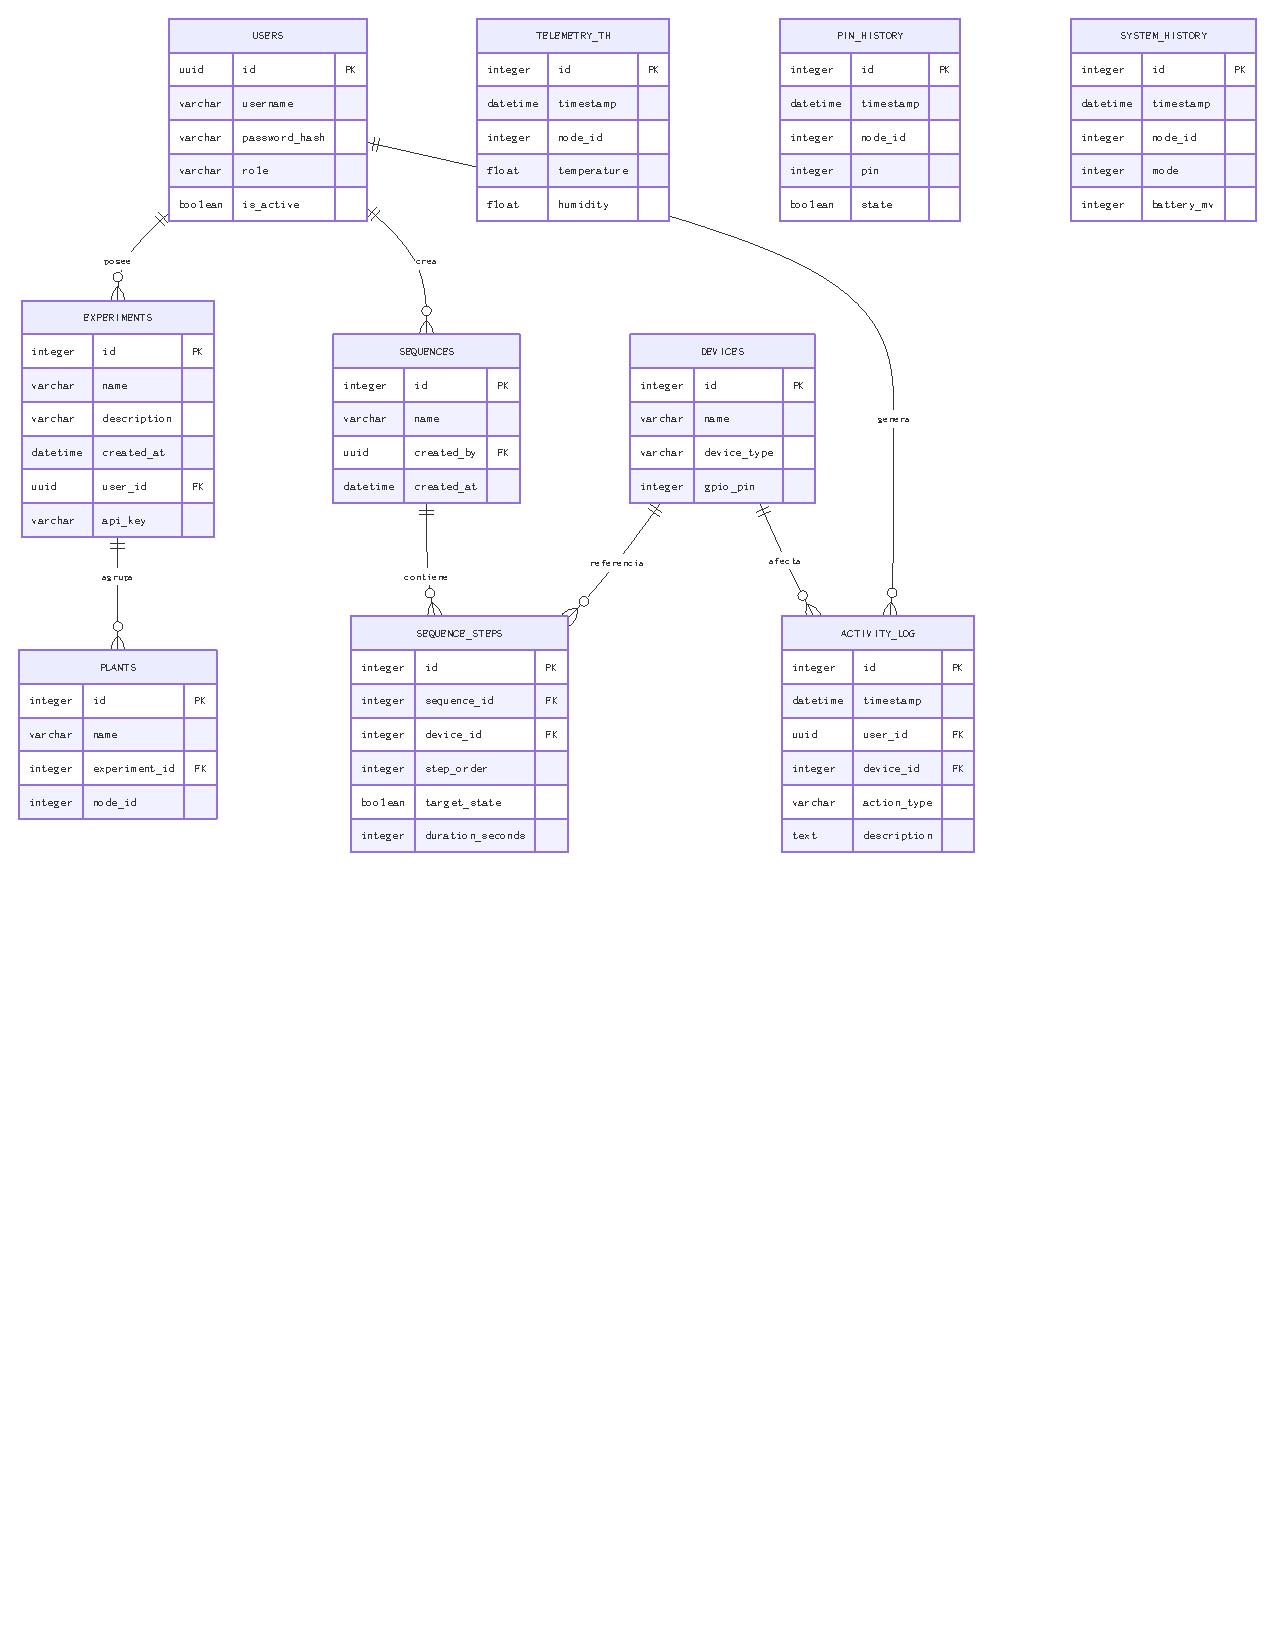
\includegraphics[width=1.05\linewidth, keepaspectratio]{16_db_schema}
    \caption{Esquema Entidad-Relación completo de \texttt{demeter\_db} (PostgreSQL 15). Generado a partir de los modelos SQLAlchemy.}
    \label{fig:anx_db_schema}
\end{figure}
\end{landscape}

\end{document}